\documentclass[a4paper, 12pt]{report}
%\setcounter{chapter}{1}
\renewcommand\thesection{\arabic{section}}
\renewcommand{\contentsname}{Cuprins}
\renewcommand{\figurename}{Figura}
\renewcommand{\tablename}{Tabel}

\setcounter{tocdepth}{6}
\setcounter{secnumdepth}{6}

\usepackage{url}
\usepackage{hyperref}
\usepackage[backend=bibtex, style=numeric, citestyle=numeric, backref=true ,sorting=none]{biblatex}
\addbibresource{bibliography.bib}

\usepackage{indentfirst}
\usepackage[nobottomtitles*]{titlesec}

\usepackage{graphicx}
\usepackage[center]{caption}
\usepackage{caption}
\usepackage{subcaption}
\usepackage[export]{adjustbox}
\graphicspath{ {./images/} }


\usepackage[margin=3.2cm]{geometry}
%\usepackage[none]{hyphenat}

\usepackage{mathtools}

\usepackage{listings}
\usepackage{color}
\usepackage{float}

\definecolor{codegreen}{rgb}{0,0.6,0}
\definecolor{codegray}{rgb}{0.5,0.5,0.5}
\definecolor{codepurple}{rgb}{0.58,0,0.82}
\definecolor{backcolour}{rgb}{0.96,0.96,0.96}

\lstdefinestyle{mystyle}{
	backgroundcolor=\color{backcolour},   
	commentstyle=\color{codegreen},
	keywordstyle=\color{blue},
	numberstyle=\tiny\color{codegray},
	stringstyle=\color{codepurple},
	basicstyle=\fontsize{10}{10}\selectfont\ttfamily,
	breakatwhitespace=false,         
	breaklines=true,                 
	captionpos=b,                    
	keepspaces=true,                 
	numbers=left,                    
	numbersep=2pt,                  
	showspaces=false,                
	showstringspaces=false,
	showtabs=false,                  
	tabsize=2
}

\lstset{style=mystyle}

\usepackage{pythonhighlight}

\usepackage{fontspec} % -> LuaLatex
\setmainfont{UT Sans}

\usepackage{setspace}
\setstretch{1.1}


\begin{document}
	
	\begin{titlepage}
	
	\vspace*{-3cm}
	\hspace{-2cm}
	
\includegraphics[width=0.8\linewidth]{./images/Logo-UT-MI-SPOT-RO}

	\begin{center}
		\Huge
		
		\vspace{2cm}
		
		\textbf{Lucrare Dizertație}
		
		\vfill
				
		\Large
		\begin{tabular}{ll}
			\textbf{Autor:}&Hanganu Bogdan\\
			\textbf{Coordonator:}&Lect. Univ. Băicoianu Alexandra
		\end{tabular}
		
		\vfill
		
		\Large
		Brașov\\
		Iulie 2022
        
	\end{center}
\end{titlepage}
	\begin{titlepage}
	
	\vspace*{-3cm}
	\hspace{-2cm}
	
\includegraphics[width=0.8\linewidth]{./images/Logo-UT-MI-SPOT-RO}
	
	\begin{center}
		\Huge
		
		\vspace{2cm}
		
		\textbf{Lucrare Disertație}
		
		\vspace{1cm} 
		
		\LARGE Detectarea emoțiilor din perspective multiple
		
		\vfill
		
		\Large
		\begin{tabular}{ll}
			\textbf{Autor:}&Hanganu Bogdan\\
			\textbf{Coordonator:}&Lect. Univ. Băicoianu Alexandra
		\end{tabular}
		
		\vfill
		
		\Large
		Brașov\\
		Iulie 2022
		
	\end{center}
\end{titlepage}
	\newpage
	\tableofcontents
	\newpage
	\pagenumbering{arabic}
	\section{Abstract}	
	Această lucrare de disertație este elaborată în jurul problematicii identificării emoțiilor unei persoane. Utilizând metode de învățare automată, datele sunt înregistrate prin intermediul unor canale multiple (audio, video și text). 
	
	Expresiile faciale, obținute prin intermediul canalului video, reflectă în mod intuitiv starea mentală a unei persoane, fiind una dintre cele mai bogate și importante forme de comunicare inter-umană. Tonalitatea vocii care se adresează în timpul comunicării ne poate oferi informații valoroase referitoare la starea de spirit. Mesajul care este transmis prin intermediul vocii, ne oferă informații referitoare la personalitatea individului, fiind de ajutor mai departe în procesul de analiză.
	Datele stocate sunt mai apoi prelucrate folosind tehnici de procesare specifice fiecărui canal. Pentru input-ul audio este folosită procesarea digitală de semnal, cu următoarele tehnici reprezentative: Transformata Fourier, Transformata Fourier pe termen scurt, Coeficienți Mels. Procesare de imagini pentru canalul video vine în adăugare cu: scalare de date, transformare imaginii în greyscale, iar pentru text este de menționat: tokenizare, lematizare. Fiecare bloc de date preprocesat în mod corespunzător canalului părinte, va trece mai departe prin pasul de recunoaștere cu ajutorul metodelor de învățare automată.
	
	
	În această lucrare au fost realizate o serie de experimente pentru: procesarea datelor, antrenarea modelelor de machine learning. Finalizarea acestor teste a avut ca urmare dezvoltarea aplicației "Multimodal Emotion Detection" care să vină în sprijinul procesului de intervievare.
	\clearpage
	
	\section{Introducere}
	Aplicația "Multimodal Emotion Detection" are ca audiență persoanele care doresc să facă o analiză a candidatului care a trecut printr-un proces de intervievare. Fiind scrisă în limbajul de programare Python, permite o manevrare concisă a datelor inregistrate, care pot fi mai apoi vizualizate de către utilizator prin intermediul framework-ului GUI (Graphical User Interface) Qt.
	
	În cadrul lucrării, se propune recunoașterea emoțiilor utilizatorului într-un mod inteligent, utilizând tehnici și metode de machine learning si deep learning. Aceste două procedee sunt subcategorii ale domeniului numit inteligență artificială (IA), domeniu care a început să se modeleze si dezvolte în funcție de nevoile oamenilor.
	
	Dezvoltarea rapidă a inteligenței artificale, "Big data science" și a tehnologiei "Block chain" a provocat multiple schimbări în structura socială umană. În majoritatea proceselor unde este nevoie de interacțiune umană, se implementează automatizări care să sporească eficiența, să folosească resursele umane, software și hardware în mod cât mai eficace. La nivel industrial, sistemele automatizate inteligente sunt deja folosite in uzine, frabici, având rolul de a asigura în permanență buna funcționare a întregului ansamblu. Atât eficiența cât și performanțele acestor sisteme sunt motivate de către costul redus de mentenanță. La un nivel mai aproape de către utilizatori, putem realiza că inteligența artificială a început tot mai des să facă parte din viața de zi cu zi, ajungând în stadiul să devină indispensabil oamenilor.
	
	În zilele noastre, interacțiunea dintre oameni și IA este în continuă creștere, ajungand să intre treptat în viața noastră de zi cu zi. De la asistenți virtuali (care au rolul de a sprijini utilizatorul prin intermediul interpretării comenziilor vocale), până la reclame personalizate, aceste sisteme inteligente interacționează din ce în ce mai mult cu ființe umane. Deoarece este un subiect în care interesul este unul foarte crescut, relația între om și mașinăria inteligentă poate să ajungă la un nivel mai inalt, prin integrarea cu emoțiile utilizatorului. Acesta este un domeniu crucial de cercetare, oferind diverse oportunități și aplicări pentru oameni.
	
	Astfel, în următorul capitol va fi explicat despre fiecare din cele trei tipuri de recunoaștere a emoției utilizate, precum și modul în care acestea interacționează cu utilizatorul. Vor fi prezentate exemple de alte categorii a recunoașterii de emoții, care nu au fost încadrate în această lucrare, precum și aplicațiile care sunt deja în domeniul comercial și sunt utilizate.
	
	\clearpage
	\section{Recunoașterea emoțiilor}
	În general, o relație între doi indivizi se bazează pe încredere și întelegere. Pentru a putea crea un parteneriat, un algoritm inteligent trebuie să fie cabail să înțeleagă emoțiile umane. Emoția este un factor important atât în comunicarea verbală, cât și în comunicarea nonverbală (gesticulare, expresiile corpului). Identificarea stărilor unei persoane poate ajuta o mașină să înțeleagă intențiile utilizatorului, în scopul de a-i oferi o interacțiune mai potrivită. Printe primele studii care au fost făcute pentru integrarea sistemelor inteligente cu emoțiile umane, aceastea s-au reflectat în identificarea emoțillor prin voce, deoarece comunicarea verbala este una dintre cele mai rapide forme de socialiare, cu cel mai mare impact in istorie.
	
	Fiind una dintre cele mai consacrate aptiduni prin care o ființă inteligentă s-a putut diferenția și avansa în lanțul trofic, comunicarea verbală reprezintă un semnal complex, în care sunt transmise informații referitoare la mesaj, legate de emițător precum și de emoțiile transmise de acesta. Fiind o serie complexa, capacitatea sistemului care face identificarea emotiilor trebuie sa fie pe măsură, pentru a analiza cu acuratețe starea subiectului, oferindu-i astfel o experiență cât se poate de autentică. Nu numai atât, utilizând o astfel de recunoaștere, poate ajuta la crearea unor interfețe usor navigabile ("Recunoașterea emoțiilor prin vorbire este deosebit de utilă pentru aplicațiile din domeniul interacțiunii om-mașină deoarece ajută la crearea unor interfețe usor de utilizat"\cite{emotion_recognition_survery}).
	
	Deoarece semnalul audio conține și alte informații precum emoția transmisă de către emițător, algortimul de recunoaștere a emoțiilor umane prin extragerea trăsăturilor acustice capturate în vorbire, devine "baza pentru realizarea unei interacțiuni om-calculator mai armonioasă și mai eficientă, având o mare importanță în cercetare, precum și aplicativă"\cite{audio_emotion_recognition0}.
	
	În cadrul aplicației, vocea utilizatorului (semnalul audio) este folosită în doua contexte. Primul este dat de către identificarea emoțiilor candidatului pe baza a diferite trăsături acustice depistate din voce iar al doilea de către identificarea cuvintelor rostite, pentru a putea fi transformate în text. Deoarece în aplicatie identificarea textului (speech-to-text) este utilizat prin intermediul unor apeluri de tip API Rest la functionalitățile oferite de către Google, accentul se va pune pe prima utilizare în lucrare. Emoțiile care pot fi identificate în cadrul acestei recunoașteri sunt următoarele: furie, dezgustare, frică, fericire, tristețe, surprindere, neutral.
	
	Seviciului oferit de către Google pentru recunoașterea textului \cite{google_speech_to_text} este folosit cu scopul de a facilita identificarea personalității și a emoției transmise în urma interviului de către utilizator. Recunoașterea emoțiilor din text este în mod fundamental o problemă de clasificare pe baza conținutului, care include noțiuniuni de procesare de text (NLP, acronim de la "natural language processing"), precum și din domeniul deep learning. Modelul utilizat pentru acest tip de predicție este "The Big Five personality traits"\cite{big_five_personality_wiki}. 
	
	\begin{figure}[h]
		\begin{center}
			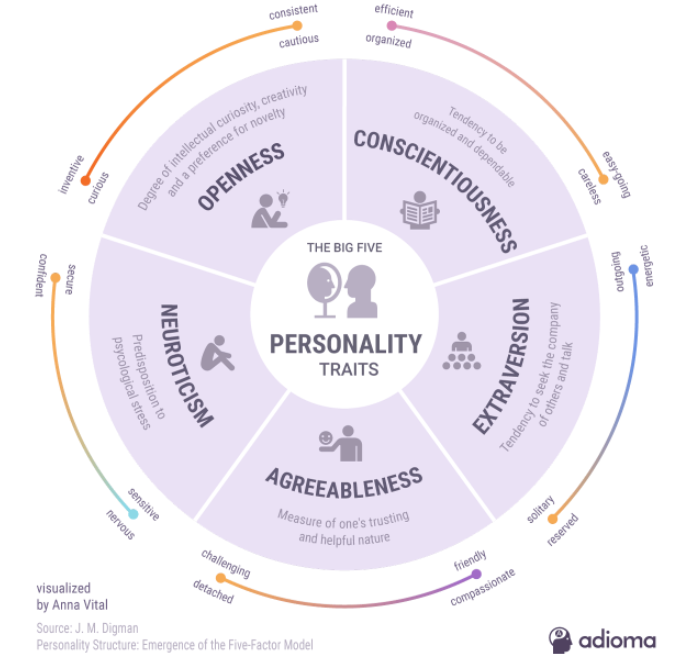
\includegraphics[scale=0.7]{images/ocean.png}
		\end{center}
		\caption{Cele cinci mari trăsături de personalitate\newline
			\hspace{\linewidth}https://blog.adioma.com/5-personality-traits-infographic/}
		\label{fig:ocean}
	\end{figure}
	
	În zilele noastre, se consideră că există 5 categorii de personalități (Figura \ref{fig:ocean}), având acronimul OCEAN. Mai jos, vom prezenta aceste personalități de bază:
	\begin{itemize}
		\item Deschidere (Openness): această trăsătură prezintă caracteristici precum imaginația și perspicacitatea. Oamenii care au punctat mai mult în această trăsătură tind să aibe o arie mai mare de interese. Sunt curioși de fire, dornici să dobândească aptitudini noi și să se bucure de orice experiență acumulată.
		
		\item Conştiinciozitate (Conscientiousness): printre caracteristicile de baza ale acestei trăsături, putem include un nivel ridicat de atenție, control bun al impulsurilor și comportamente care coduduc spre îndeplinirea obiectivelor. Oamenii care se încadrează acestei categorii tind să fie mai organizați și atenți la detalii. Ei planifică din timp, se gândesc la modul în care comportamentul lor îi afectează pe alții și sunt atenți la termenele limită.
		
		\item Extraversie (Extraversion): se caracterizează prin excitabilitate, sociabilitate și cantități mari de expresivitate emoțională. Oamenii care au un nivel ridicat de extraversie tind să capete energie în situații sociale. A fi în preajma altor persoane îi ajută să se simtă plini de energie și entuziasm.
		Oamenii care au un nivel scăzut de extraversie (sau introvertiți) tind să fie mai rezervați și au mai puțină energie în mediile sociale. În urma evenimentelor sociale se pot simți extenuați, iar introvertiții necesită adesea o perioadă de singurătate și tăcere pentru a își putea "reîncărca bateriile".
		
		\item Agreabilitate (Agreeableness ): pentru această personalitate, sunt incluse atribute precum încrederea, altruismul, bunătatea, afecțiunea și alte comportamente pro-sociale. Oamenii cu grad ridicat de agreabilitate tind să fie mai cooperativi, în timp ce aceia care au punctat mai slab pentru acest atribut, tind să fie competitivi și uneori chiar manipulativi.
		
		\item Nevrotism (Neuroticism): este un atribut caracterizat prin tristețe, melancolie și inconsevcență emoțională. Persoanele care au această trăsătură au tendința de a experimenta schimbări de dispoziție, anxietate, iritabilitate și tristețe. Aceia care au punctat scăzut în acest caz, tind să fie mai stabili și rezistenți emoționali.
	\end{itemize} 
	
	Nu în cele din urmă, dupa procesul de recunoaștere a trăsăturilor și emoțiilor transmise din voce, mai apoi interpretate în mod contextual prin procesare de text, urmează recunoașterea emoțiilor din cadrul expresiilor faciale. Pentru a putea fi în stare să facem o astfel de analiză, este nevoie identificarea unui chip uman (în engleză "face detection"). Pentru a facilita acest proces, prin intermediual camerei web care ne oferă flux de date video, biblioteca OpenCv\cite{open_cv} ne oferă suport pentru mijloace de identificare a fețelor candidaților. Având acest rezultat intermediar, este posibilă recunoașterea emoțiilor pe baza expresiilor faciale. Principalele stări emotive din cadrul fluxului video sunt aceleasi ca cele din audio.
	
	Făcând un ansamblu al componentelor descrise mai sus, acestea se unifică în ceea ce vom numi "Modulul de intervievare". În cadrul acestui modul, predicțiile pentru componentele audio și video sunt făcute live, iar in cazul textului, este realizat la final pentru a avea o cantitate mai ridicată de date, obținânand astfel o predicție cât mai aproape de adevăr.
	
	Tipurile de identificare a emoțiilor utilizate și descrise mai sus sunt doar câteva modele existente prin care o aplicație/mașină inteligentă poate interacționa în mod personalizat cu utilizatorul. Printre alte tipuri care merită menționate se enumeră gesturile corpului (limbajul corpului), fiind un subiect mai puțin explorat. Chiar dacă este un aspect important al psihologiei umane, primule studii moderne au devenit populare debia în 1960. Probabil cea mai importantă lucrare publicată înainte de secolul al XX-lea a fost "Expresia emoțiilor la om și la animale", scrisă de Charles Darwin \cite{human_body_lang_darwin}.
	
	\subsection{Soluții existente în predicția emoțiilor umane}
	În acest domeniu, după o cercetare a pieței care construiesc software-uri în jurul predicției emoțiilor, putem considera aplicațiile menționate mai jos ca fiind similare cu cea prezentată în această lucrare:
	\begin{itemize}
		\item Noldus Solutions Emotion Analysis cu "FaceReader™" \cite{noldus}: este un software specilizat pe analizarea datelor de tip imagine (atât din video cât și statice). Este un sistem robust, capabil să recunoască un număr de proprietăți specifice în imaginile faciale, inclusiv cele șase expresii de bază sau universale: fericit, trist, furios, surprins, speriat și dezgustat.
		\item iMotions cu "Facial Expression Analysis" \cite{imotions}: este un software specializat atât în analiza imaginilor cât și a datelor biosenzoristice. Modulul oferă 20 de măsuri de expresie facială (unități de acțiune), 7 emoții de bază, repere faciale, indici comportamentali, cum ar fi orientarea capului și atenția.
	\end{itemize}
	
	Diferența pe care o aduce aplicația prezentată în lucrare curentă, "Multimodal Emotion Detection",  este reprezentată de capacitate recunoașterii în timp real a emoțiilor prin intermediul altor input-uri, precum și a feedback-ului constant. Un alt aspect important prin care se diferențiază aplicația în cauză este dat de "Modulul de vizualizare a raportului", prin care se poate vedea la fiecare segment de date, textul care a fost spus, emoțiile prezise din input-ul audio, video, cât și o spectogramă pentru intervalul selectat de date în care s-a efectuat predicția.
	
	Gama de public cărui este adresată această aplicație este reprezentată în general de persoanele care trec prin procesul de intervievare. Dar asta nu înseamnă că recunoaștere emoțiilor se limitează la această aplicativitate. Mai jos sunt listate o serie de utilizări:
	\begin{itemize}
		\item Marketing personalizat: un studiu realizat de OneSpot Research a arătat că în proporție de 88\% dintre consumatorii chestionați au declarat că un conținut mai personalizat îi face să se simtă mai bine cu privire la un anumit brand.
		\item Diagnostic medical: o aplicabilitate în care poate sprijinii medicii cu diagnosticarea afecțiunilor nevrotice precum depresia sau demența, utilizând analiza vocală
		\item Educație: diferite software-uri didactice în variantă prototip au fost elaborate pentru a se acomoda la emoția copiilor. Când copilul exprimă frustrare pentru că o sarcină este prea simplă sau dificilă, programul se adaptează astfel încât sarcina să se schimbe într-o formă mai adecvată.
	\end{itemize}
	
	În următoarele capitole, vom trece printr-o inițiere în inteligența artficială, procesare digitală de semnal, procesare de imagini și text, toate aceste componente fiind esențtiale în dezvoltarea aplicației de față. Având aceste cunoștiințe asimilate, următoarele subiecte propuse care vor fi comentate se vor afla în sfera tehnologiilor utilizate, fără de care nu s-ar fi putut crea aceste teste, precum și aplicația "Multimodal Emotion Detection". 
	\clearpage
	
	\section{Noțiuni teoretice}
	\subsection{Inteligența artificială}
	David Fogel a definit inteligența ca fiind "abilitatea unui sistem de a se adapta astfel încât să își poată îndeplini scopurile cu succes". Astfel, o mașinărie programată și dotată cu inteligență artificială este un sistem complex capabil să facă decizii, fără nevoia intervenției unei persoane, simulând inteligența umană. Perturbarea funcționării unui astfel de sistem poate altera fluxul evenimentelor în luarea deciziilor, ajungând astfel la rezultate nejustificabile. Principalele subcategorii ale IA sunt: machine learning și deep learning.
		
	\begin{figure}[h]
		\begin{center}
			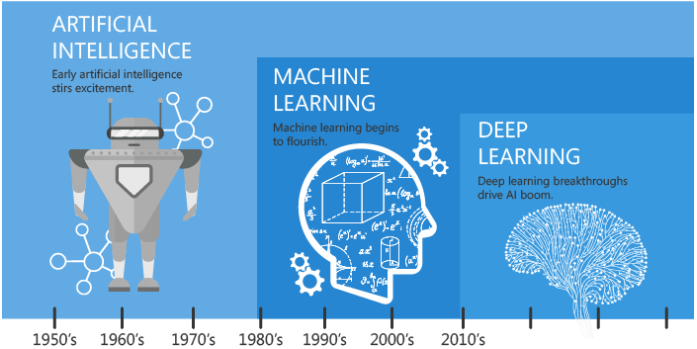
\includegraphics[scale=0.7]{images/AI_ML_DL.png}
		\end{center}
		\caption{Dezvoltarea inteligenței artificiale\newline
			\hspace{\linewidth}https://towardsdatascience.com/artificial-intelligence-vs-machine-learning-vs-deep-learning-2210ba8cc4ac/}
		\label{fig:AI_ML_DL}
	\end{figure}
	
	Așa cum se observă în Figura \ref{fig:AI_ML_DL}, putem afirmă că inteligența artificială este un termen mai vast care cuprinde celelalte două subcategorii. Aplicațiile care utilizează acest tip de tehnologie imită funcțiile cognitive pe care oamenii le asociază cu mințile umane, cum ar fi învățarea sau rezolvarea anumitor probleme.
	
	Machine learning înglobează algoritmii clasici pentru diferite tipuri de sarcini, precum regresia sau clasificarea. Acești algoritmi sunt dependenți în permanență de datele utilizate în procesul antrenării. Cu cât sunt mai multe date și cu cât aceste date sunt mai relevante pentru problema care încearcă să se soluționeze, randamentul acestora va crește. Antrenarea lor reprezintă cel mai important pas, deoarece în acest proces, se presupune minimizarea funcției de eroare (loss function). Rolul acesteia este de a stabili valorile de adevăr între ce a fost prezis, și adevărata clasă a datelor respective. În raport cu răspunsul funcției de eroare în cauză, anumite valori denumite greutăți (weights) vor fi actualizate.
	
	În învățarea automată există două categorii de date din care se poate învăța: date etichetate și date neetichetate. În prima categorie, atât parametrii de intrare cât și cei de ieșire sunt într-o formă ușor de citit pentru mașină, fiind nevoie de o cantitate mare de timp pentru a putea eticheta. În cazul datelor neetichetate, este nevoie de o soluție mai complexă pentru a putea utiliza acele informații. Astfel, reies la suprafață trei tipuri de învățare în machine learning:
	\begin{itemize}
		\item Învățare supervizată: este una din cele mai de bază tipuri de învățare automată. Chiar dacă este antrenat cu date etichetate, acest gen de învățare este unul foarte puternic. Se folosește un set de date (sau o parte din acest set de date, în general referindu-ne ca set de antrenare), care servește algoritmului cu scop de pregătire, iar alt set de date pentru a testa performanțele modelului.
		\item Învățare nesupervizată: principalul avantaj al acestei categorii este capacitatea algoritmilor de a lucra cu seturi de date neetichetate, eficientizând timpul programatorului. Permit astfel algoritmilor să exploreze și să găsească diferite șabloane și asocieri în seturile de date.
		\item Învățare prin "întărire" (reinforcement): se inspiră direct din modelul în care ființele umane învață din experiențele din viața de zi cu zi. Dispune de un algoritm care se îmbunătățește pe sine și învață din situații noi folosind o metodă de "încearcă și greșește" (în engleză trial and error). Rezultatele favorabile sunt încurajate sau "întărite", iar rezultatele greșite sunt descurajate sau "pedepsite".
	\end{itemize}
	
	Referitor la Figura \ref{fig:AI_ML_DL}, se poate constanta că machine learning este un domeniu destul de îmbătrânit, care încorporează metode și algoritmi, precum: Naive Bayes Classifier, Support Vector Machine, Random Forest. 

	Recent, în industria inteligenței articiale, a apărut conceptul de deep learning, care asamblează rețele artificiale neurale cu mai multe straturi. Deep learning poate fi definit ca un subset al învățării automate, care încearcă rezolvarea problemelor mai complexe prin găsirea unor diferite șabloane (pattern-uri) în date, acestea pentru oameni fiind insesizabile cu ochiul liber.

	Avantajul pe care îl aduc aceste tipuri de rețele față de cele tradiționale, este dat de eliminarea necesității de a extrage caracteristici din cadrul setului de date. Rezultatul extragerii caracteristicilor din setul de date definește o reprezentare abstractă a datelor. Acest proces este de obieci destul de complicat, care necesită cunoștințe detaliate în aria specifică a problemei care se încearcă soluționarea. Pasul extragerii trebuie revizuit de multiple ori, testat și rafinat pentru a obține rezultate optime.
	
	\clearpage
	
	\begin{figure}[h]
		\begin{center}
			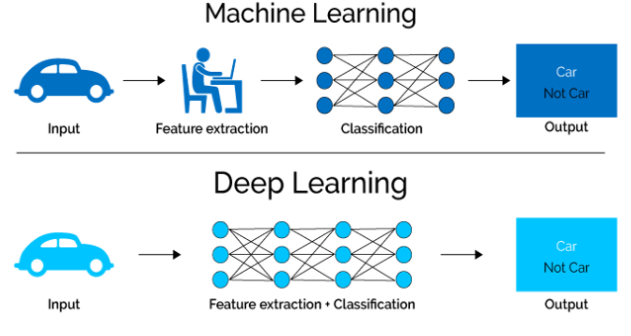
\includegraphics[scale=0.7]{images/ML_DL.png}
		\end{center}
		\caption{Analogie învățare automată și învățare profundă\newline
			\hspace{\linewidth}https://www.researchgate.net/figure/Comparison-between-ML-and-Dl-algorithm\_fig5\_344628869/}
		\label{fig:ML_DL}
	\end{figure}

	Pe de altă parte, în Figura \ref{fig:ML_DL}, se poate observa cum în cazul învățării profunde, pasul de extragere a caracteristicilor nu mai este necesar să fie executat de către programator, ci devine parte în procesul de antrenare a rețelei artificiale. Datele sunt brute și abstractizate astfel încât să poată fi memorate de diversele straturi ale algoritmului inteligent. Această reprezentare comprimată a datelor de intrare este utilizată pentru a construi rezultatul.

	Cu ajutorul rețelelor neurale profunde, acestea au făcut posibilă înțelegerea a seturilor de date complexe, precum semnalul audio reprezentând vocea umană, expresiile faciale și textul asociat cu fraze. Datele de antrenare folosite (care vor fi prezentate în capitolele următoare), sunt etichetate, făcând astfel posibilă identificare emoțiilor și a personalității candidatului. În secțiunea următoare, vom prezenta în mod minimalist modelele utilizate în aplicație:
	\begin{itemize}
		\item Rețele neurale convoluționale
		\item Rețele neurale recurente
	\end{itemize} 

	\clearpage
	\subsubsection{Rețele neurale convoluționale}
	O rețea neurală convolutională este un de algoritm inteligent care face parte din clasa modelelor deep learning. În general folosite în vederea artificială (computer vision), CNN (convolutional neural network) primește ca date de intrare, în majoritatea cazurilor, imagini (sau date care au fost structurate sub forma imaginilor), iar în urmă diferitelor operațiuni, se vor găsi pattern-uri în datele de antrenare, nevizibile unei persoane în mod natural. Sunt distinse printre alte tipuri de modele datorită performanțelor ridicate cu date care provin din: imagini, vorbit 	sau semnal audio.
	
	Din punct de vedere structural, o rețea neurală convolutională este alcătuită din următoarele componente:
	\begin{itemize}
		\item \textbf{Date de intrare}: cum este menționat mai sus, input-ul poate să provină din mai multe categorii, având și canale diferite de culori. Nu există o limită privind dimensiunea datelor, deoarece, scopul întregului proces este de a reduce dimensionalitatea, păstrând datele într-o formă compresată, fără pierderi de informații.
		\item \textbf{Strart(uri) de convoluție}: este elementul de bază al unei astfel de rețele, fiind locul în care majoritatea calculelor au loc. În funcție de dimensionalitatea datelor (matrici 2d sau 3d), va avea loc operația de convoluție, cu ajutorul unor măști (kernel). În urma acestui proces, se vor extrage anumite trăsături importante din cadrul datelor de intrare, care vor ajuta în determinarea apartenenței la o anumită clasă. De exemplu, printr-o speculație, putem considera din Figura \ref{fig:cnn}, în urma unui proces de convoluție, că se poate determina dacă piciorul mamiferului este sau nu al unei zebre. În urmă acestui proces, în funcție de numărul filtrelor, pasul (stride) și padding, se obțin hărți ale caracteristicilor (feature maps).
		\item \textbf{Strat(uri) de pooling}: au rolul de a reduce substanțial dimensiunea spațială, scăzând cantitatea de parametrii utilizați pentru calcule în rețea. Totodată, poate controla și "supra-adaptarea" (overfitting) rețelei. Printre tipurile de straturi de pooling, putem menționa următoarele:
		\begin{itemize}
			\item \textbf{Max pooling}: fiind cea mai comună abordare, deoarece oferă cele mai bune rezultate, max pooling va selecta elementul maxim din harta caracteristicilor (porțiunea filtrată de către mască)
			\item \textbf{Average pooling}: cum reiese și din nume, va selecta valoare medie din porțiunea filtrată de mască
		\end{itemize}
		\item \textbf{Strat(uri) de conectare}: sunt folosite cu scopul conectării neuronilor către stratul de ieșire, unde în funcție de valorile ponderilor fiecărui neuron în parte, se va putea face calculul posibilității apartenenței la o anumită clasă
	\end{itemize} 
	
	\clearpage
	\begin{figure}[h]
		\begin{center}
			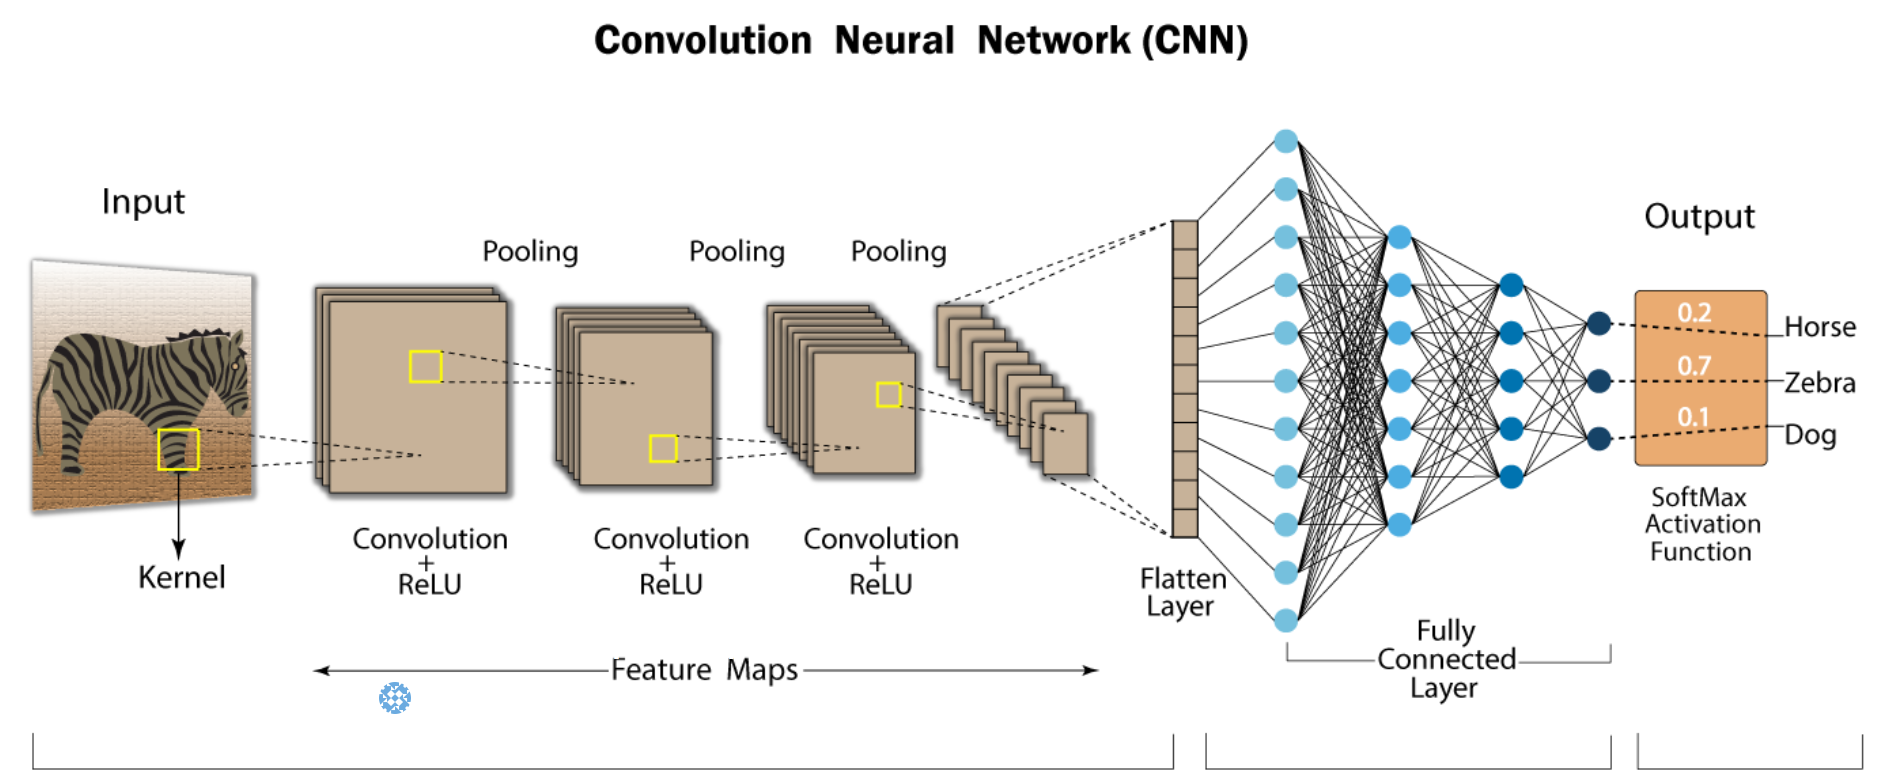
\includegraphics[scale=0.29]{images/cnn.png}
		\end{center}
		\caption{Rețea neurală convoluțională\newline
			\hspace{\linewidth}https://developersbreach.com/convolution-neural-network-deep-learning/}
		\label{fig:cnn}
	\end{figure}
	
	Împreună cu informațiile pe care le-am dobândit în urmă prezentării legate de rețelele neurale convolutionale, putem comenta asupra Figurii \ref{fig:cnn}. Din datele folosite pentru antrenare, filtrele aplicate succesiv ne vor ajută să găsim caracteristici. Transmise mai departe către stratul conectat, se va putea face interpretarea rezultatului, în funcție de gradul de apartenența la fiecare clasă în parte. Rezultatul va fi exprimat în procentaj, iar output-ul cu procentajul cel mai ridicat va exprima clasa decisă.
	
	În contextul aplicației "Multimodal Emotion Detection", acest tip de algoritm a fost utilizat cu preponderență în cazul identificării emoțiilor fluxul video și audio. Prin intermediul acestor rețele, în imaginile procesate din input-ul video/audio se vor găsi diferite asemănări, neuronii excitându-se atunci când un șablon recunoscut este detectat, fiind posibil ca emoțiile candidatului unui interviu să fie recunoscute. 
	
	\clearpage
	\subsubsection{Rețele neurale recurente}
	Rețelele neurale recurente sunt un tip robust de rețea neurală, folositoare pentru procesarea datelor secvențiale, ordinea lor având importantă. Derivate din rețelele cu propagare înainte (feedforward), RNN-urile (recurrent neural network) prezintă un comportament asemănător cu cel al creierului uman.

	La fel că ceilalți algoritmi de deep learning, rețelele neurale recurente sunt relativ vechi, fiind concepute în 1980, dar doar în ultimii ani a fost descoperit cu adevărat potențialul acestora. Creșterea în puterea computațională, accesul la cantități masive de date pe care le putem utiliza și apariția straturilor cu memorie lungă pe durata scurtă (long short-term memory), au adus RNN-urile în prim plan.

	După cum menționează Lex Fridman ("Ori de câte ori există o secvență de date temporale, unde conținutul spațial este mai important decât cel al fiecărui cadru individual"), rețelele neurale recurente au oferit suport pe parcursul lucrării pentru predicția datelor cu strânsă legătură temporală. Aceste rețele și-au îndeplinit scopul în aplicația "Multimodel Emotion Recognition" deoarece atât datele audio cât și cele scrise depind de ordinea lor în timp.

	Datele secvențiale sunt doar date ordonate în funcție de un anumite criteriu. Spre exemplu, putem menționa că date secvențiale, datele financiare sau chiar secvența de ADN. Cele mai populare date secvențiale sunt reprezentate de către seria temporală, în care sunt enumerate în ordine cronologică. Datele provenite din vorbit, care sunt utilizate în aplicație pentru a prezice emoția, sunt adecvate acestei rețele datorită sortării cronologice standard.

	Pentru a înțelege arhitectură acestor rețele, trebuia mai întâi să avem cunoștințe referitoare la mecanismul utilizat de această rețea, propagarea înainte. Într-o rețea neurală feed-forward, informațiile se mișcă doar într-o singură direcție: de la stratul de intrare, prin straturile ascunse, până la nivelul de ieșire. Informația se deplasează direct prin rețea și nu atinge același un neuron de două ori. Rețelele simple nu au niciun mecanism de memorare, cu privire la intrarea pe care o primesc, fiind slabe în a prezice ce urmează. Într-un RNN, informația circulă sub formă unei bucle. Când se ia o decizie, se va evalua input-ul curent cât și ce a învățat din experiențele anterioare.
	
	\begin{figure}[H]
		\begin{center}
			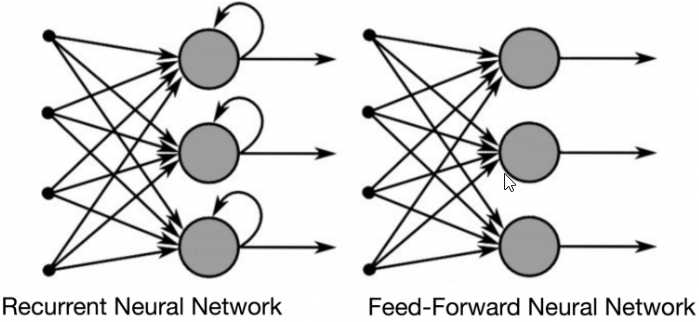
\includegraphics[scale=0.47]{images/fwd_recc.png}
		\end{center}
		\caption{Propagare recurentă și înainte\newline
			\hspace{\linewidth}https://builtin.com/data-science/recurrent-neural-networks-and-lstm/}
		\label{fig:fwd_recc}
	\end{figure} 

	În Figura \ref{fig:fwd_recc}, este ilustrată diferența dintre fluxul de intrare într-o rețea neurala recurentă și o rețea cu propagare înainte.
	
	O rețea neurala feed-forward atribuie, că toți ceilalți algoritmi de deep learning, o matrice de ponderi care va fi aplicată asupra datelor de intrare, urmând mai apoi să producă rezultatul. Totodată, va avea loc procesul de propagare înapoi (back propagation) petru actualizarea ponderilor. 
	
	Propagarea înapoi este utilizată pentru a calcula gradientul unei funcții de eroare în raport cu ponderile unei rețele neurale. Algoritmul își parcurge calea înapoi prin straturile rețelei, calculând derivatele parțiale ale ponderilor. Această tehnică este folosită pentru a reduce marjele de eroare în timpul antrenamentului.
	
	Mai jost sunt listate diferențele dintre o rețea normală și una recurentă, în contextul celor două propagări:
	\begin{itemize}
		\item Propagarea înainte: în acest pas, RNN-ul va înainta prin aplicarea ponderilor și pentru datele anterior procesate
		\item Propagarea înapoi: o astfel de rețea modifică greutățile atât prin gradient descent cât și prin propagarea inversă în timp (back propagation through time)
	\end{itemize}
	
	Principalele neajunsuri în cazul acestor algoritmi au apărut datorită gradientului. Primul este denumit "Explozia gradientului" (Expploading Gradient) și apare în cazurile când se asignează valori semnificativ de mari pentru ponderi. Această este ușor rezolvabilă prin trunchierea/plafonarea acestuia. A două problemă o reprezintă "Gradientul care dispare" (Vanishing Gradient), care apare atunci când valorile gradienților sunt prea mici, iar modelul încetează să învețe ori o face într-un timp prea mare. Pentru a rezolva această problema, au fost introduse straturile LSTM (Long Short-Term Memory).
	
	LSTM sunt o extensie pentru RNN-uri, unde se prelungește durata memoriei interne. Sunt folosite că elemente de baza pentru straturile rețelelor recurente. LSTM-urile asociază încă un set diferit de ponderi folosit pentru a oferi un grad de importanță asupra datelor noi. În funcție de aceste ponderi, datele noi vor putea impacta sau nu pe cele deja existente.
	
	Aceste straturi oferă suport rețelelor recurente să-și "amintească" input-urile pentru o perioada mai lungă de timp. Funcționalitate lor este asemănătoare cu cea a unui calculator, având capabilități de citire, scriere sau ștergere. Această memorie poate fi privită precum o celulă cu porți, care decide dacă să stocheze informația, să o șteargă, în funcție de importanța pe care trebuie să o acorde.
	
	Antrenarea utilizând astfel de rețele poate deveni una costisitoare datorită cantităților mari de date și a complexității calculelor. Procesorul central devine depășit de această ușoare, iar timpul necesar antrenării pentru acești algoritmi poate crește. Soluționarea în acest caz vine prin utilizarea procesorului grafic, acolo unde placă video permite acest lucru.
	
	\clearpage
	\subsubsection{Antrenare utilizând procesorul grafic}
	Procesorle grafice (graphical proccesing unit), dezvoltate inițial pentru accelerarea procesării grafice, pot îmbunătăți performanțele calculelor realizate într-o rețea neurală cu mai multe straturi. Au devenit o parte esențială a  infrastructurii inteligenței artificiale, iar procesoarele grafice noi au devenit specializate în acest domeniu.
	
	Principalul beneficiu al utilizării procesorului grafic este dat de paralelizarea sau procesarea simultană a datelor. Există patru tipuri de arhitecturi folosite pentru procesarea datelor în mod pparalel :
	
	\begin{itemize}
		\item Instrucțiune unică, date unice
		\item Instrucțiune unică, date multiple
		\item Instrucțiuni multiple, date unice
		\item Instrucțiuni multiple, date multiple
	\end{itemize}
	
	Scopul inițial al procesoarelor grafice erau pentru procesarea video, astfel solicitând utilizatorii să înțeleagă limbaje specifice precum C. În 2007, odată cu lansarea framework-ului NVIDIA CUDA \cite{cuda}, aria utilizării procesoarelor grafice a fost extinsă. CUDA se bazează pe limbajul de programare C și oferă un API (application programmin interface) pe care dezvoltatorii îl pot folosi pentru a aplica puterea de computație oferită de placa video în sarcinile de machine learning.
	
	Odată ce NVIDIA a introdus CUDA, au fost dezvoltate mai multe framework-uri pentru învățarea profundă, precum PyTorch și TensorFlow. Aceste tehnologii se folosesc de capabilitățile oferite de CUDA, oferind o accesibilitate mai mare pentru implementările moderne de deep learning.
	
	Procesoarele grafice pot efectua calcule simultan. Acest lucru permite distribuirea proceselor de instruire și poate accelera semnificativ operațiile de învățare automată. Folosind numărul mare de nuclee, putem utiliza mai puține resurse fără a sacrifica eficiența sau puterea.
	
	Când se definește o arhitectură pentru rețelele deep learning, următorii factori pot influență decizia de a utiliza sau nu un procesor grafic:
	\begin{itemize}
		\item Lățimea bandei de memorie: datorită memoriei video dedicată (VRAM), GPU-urile pot oferi lățimea de bandă necesară pentru a acomoda seturi de date
		\item Dimensiunea setului de date: procesoarele grafice legate în paralel scalează mult mai rapid decât procesoarele centrale, permițând procesarea a unor seturi de date masiv din punct de vedere cantitativ
	\end{itemize}
	
	Datorită puterii de procesare a plăcilor grafice, modelele de deep learning folosite în aplicație au fost antrenate cu ajutorul procesorului grafic. Placa video utilizată în cauză este un GeForece RTX 2060 (ediția laptop), oferind 1920 procesoare CUDA și 240 procesoare Tensor.
	\clearpage

	\subsection{Procesare digitală de semnal}
	Aceste tehnici complexe de procesare au fost utilizate în aplicație pentru identificarea emoției din voce. Această procesare nu va identifica cuvintele rostite de candidat, ci va încerca în funcție de anvelopa acustică, să determina starea persoanei care este intervievată.

	În mod natural, vocea este transmisă urechii umane printr-o undă acustică care se deplasează prin intermediul aerului, cu viteză sunetului. Din momentul în care este înregistrată de către un microfon, sunetul este transmis printr-un fir ca un semnal electric care se deplasează cu viteză luminii. Pentru a face acest eveniment posibil, semnalul acustic generat de corzile vocale umane trebuie mai întâi transformat într-un semnal electric și apoi convertit într-o formă acustică, pentru a putea fi înțeles de către oameni. Semnalul electric convertit este în mod convențional într-o formă analogică. Adică este reprezentat ca o tensiune care variază continuu într-un interval dat (0 și 1). Datorată degradării semnalului electric în cazul stocării, a deplasării acestuia pe distanțe lungi sau a procesării de către un calculator, se preferă transformarea lui într-o formă digitală.

	Indiferent de domeniul utilizat (timpului sau frecvențelor), următorii termeni prezentați mai jos vor ajută în înțelegerea procesului de identificare a emoțiilor:
	
  	\begin{itemize} 
  		\item Rata de eșantionare (Sample rate): reprezintă numărul de date (sample-uri) care sunt înregistrate într-o secundă. Cu cât avem rată de eșantionare mai mare, cu atât calitatea semnalului va fi mai ridicată. Spre exemplu, rata de eșantionare folosită în general pentru scrierea CD-urilor cu muzică este de 44.1 KHz (kilo Hertzi). Asta înseamnă că o dată la o secundă, 44100 de date sunt înregistrate, pe care le putem studia. 
  		\item Fereastră (Window): semnalul poate fi segmentat într-un numărul egal de sample-uri 
  		\item Numărul de linii spectrale: simbolizează numărul de frecvențe identificate în urmă transformării din domeniul timpului în cel al frecvențelor 
  	\end{itemize} 
 	 Datele înregistarte de către microfon se vor află în domeniul timpului. În această sferă, principalul neajuns este reprezentat de insuficiența de operații folositoare pe care le putem utiliza în identificarea emoțiilor vocii. Pentru a satisface cerințele necesare analizei sentimentelor din voce, vom efectua trecerea din domeniul timpului în cel al frecvențelor, utilizând Transformata Fourier \cite{ft}. 
  
 	 \clearpage 
  	\subsubsection{Transformata Fourier} 
  	Fiind folosită în multiple domenii precum procesarea imaginiilor, studiul semnalelor (incluzând cele acustice), transformata Fourier este un procedeu matematic care ne ajută la trecerea unui semnal din domeniul timpului în cel al frecvențelor. Avantajul analizei în acest domeniu este dat gama diversificată de informații precum și de operații pe care le putem folosi. 
  	
  	O puternică unealtă matematică, transformata Fourier (Jean-Baptiset Joseph Fourier) asumă faptul că un semnal poate fi descompus ca o suma de sinusuri/cosinusuri.
	
	\begin{figure}[h]
		\begin{center}
			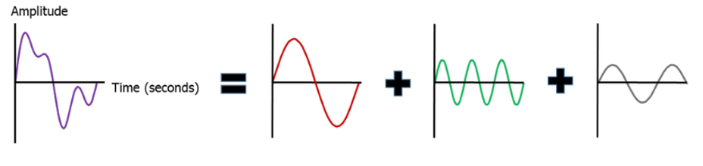
\includegraphics[width=\linewidth]{images/signals.png}
		\end{center}
		\caption{Semnal ca fiind o sumă de sinusuri\newline
			\hspace{\linewidth}https://community.sw.siemens.com/s/article/what-is-the-fourier-transform}
		\label{fig:singal_to_sinuses}
	\end{figure}

	Din Figura \ref{fig:singal_to_sinuses} se poate observa cum un semnal definit de amplitudine și timp, poate fi descompus într-o sumă de sinusuri, de frecvențe diferite.
	
	\begin{figure}[H]
		\begin{center}
			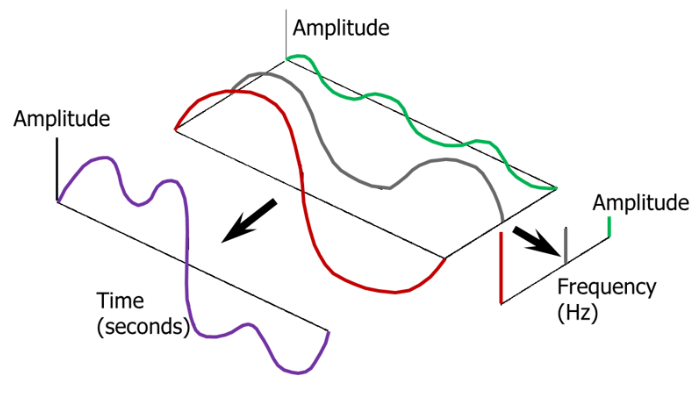
\includegraphics[scale=0.7]{images/FT_time_to_freq}
		\end{center}
		\caption{Domeniul frecvențelor \newline
			\hspace{\linewidth}https://community.sw.siemens.com/s/article/what-is-the-fourier-transform}
		\label{fig:signal_to_freq}
	\end{figure}

	Datorită motivelor enunțate în pagină anterioară care justifică necesitatea transformării în domeniul frecvențelor, vom explica acest fenomen cu ajutorul Figurii \ref{fig:signal_to_freq}. Putem observa că semnalul reprezentat de culoarea mov este compus din alte trei semnale. În urmă aplicării transformatei Fourier peste acest semnal, liniile spectrale vor reprezenta principalele frecvențe recunoscute.

	Din punct de vedere matematic, transformata Fourier este:
	\begin{equation}
		\label{ft_equation}
		S_x(f) = \int_{-\infty}^{+\infty} x(t)e^{-j2 \pi ft} dt
	\end{equation}
	
	unde $S_x(f)$ reprezintă frecvența măsurată în Hz iar $x(t)$ este semnalul în domeniul timpului. Rezultatul acestei operații este un număr complex (spre exemplu $a + bj$ este un număr complex întrucât a reprezintă partea reală iar b partea imaginară).
	
	\subsubsection{Transformata Fourier pe termen scurt}
	Adesea, transformata Fourier este evitată în a fi folosită în forma ei simplă în practică. Motivul este dat de variațiile prea bruște și multiple pe care semnalul le poate avea în domeniul timpului. Interpretarea unui semnal dintr-un singur segment devine problematică și costisitoare din punct de vedere al performanțelor. O soluție fezabilă este segmentarea semnalului în intervale mici, care mai apoi vor fi interpretate în mod individual. Această tehnică poartă numele de transformata Fourier pe termen scurt (short time Fourier Transform, STFT).
	
	\begin{figure}[H]
		\begin{center}
			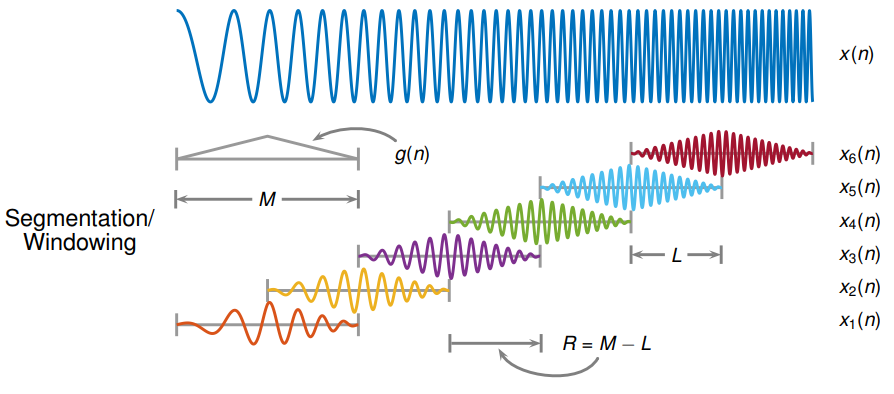
\includegraphics[width=\linewidth]{images/windowing.PNG}	
		\end{center}
		\caption{Domeniul frecvențelor \newline
			\hspace{\linewidth}https://nl.mathworks.com/help/signal/ref/stft.html}
		\label{fig:windowing}
	\end{figure}

	După cum se poate observa în Figura \ref{fig:windowing}, se aplică succesiv transformata Fourier pe segmente mici de date. Lungimea unui segment este aleasă în mod arbitrar, dar se recomandă să se folosească puteri ale lui 2, pentru a spori eficiența algoritmului. Acest proces este documentat ca fiind etapa de "windowing". O proprietate specială pe care o are acest procedeu este dat de intercalarea segmentelor. Prin utilizarea ferestrei în mod intercalat, vom avea posibilitatea de a obține valorile frecvențelor într-un mod mai determinist.
	
	\begin{figure}[H]
		\begin{center}
			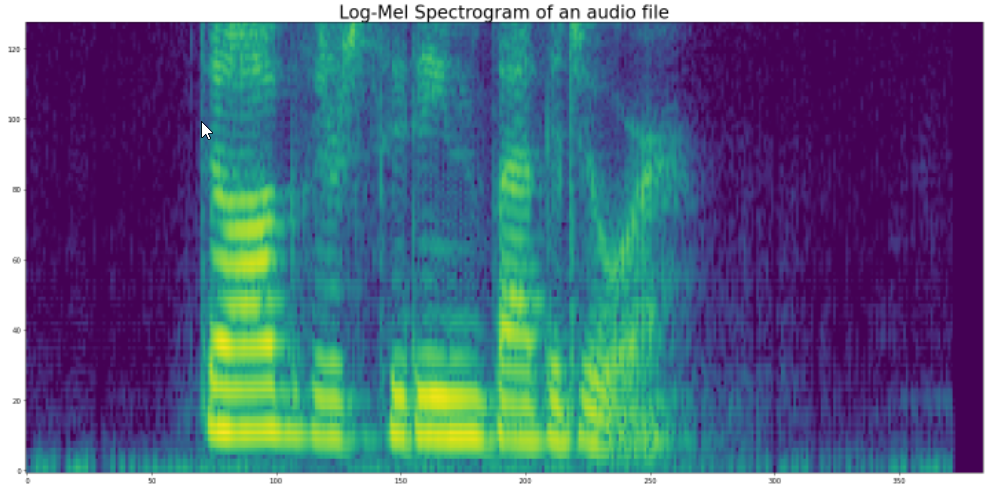
\includegraphics[width=\linewidth]{images/spectogram.PNG}	
		\end{center}
		\caption{Spectograma unui fișier audio folosit în antrenare}
		\label{fig:spectogram}
	\end{figure} 

	Rezultatul obținut în urma aplicării transformatei Fourier pe termen scurt poate fi interpret sub forma unui grafic care poartă denumirea de spectogramă sau cascadă (waterfall). În exemplul din Figura \ref{fig:spectogram}, într-un spațiu cartezian XOY, axa OX reprezintă timpul iar cealaltă axă arată puterea lui. În funcție de intensitatea culorilor, putem determina degradarea precum și anvelopa acustică a semnalului sonor.
	
	\clearpage
	\subsection{Tehnologii utilizate}
	"Multimodal Emotion Detection" este o aplicație în care au fost folosite o serie de tehnologii. Aceste unelte fac posibilă atât navigarea printr-o interfață grafică prietenoasă utilizatorului, cât și cele mai importante funcționalități de bază, precum identificarea emoțiilor. Este o aplicație desktop, care oferă utilizatorului posibilitatea de a revizui un interviu, cu scopul identificării unor momente cheie, care au fost omise în procesul interviului.
	
	În funcție de cerințele și necesitățile aplicației, direcția aleasă în materie de tehnologii și limbaje de programare trebuie să fie una justificabilă. Așteptările construite în faza de proiecție, testare sau design trebuie menținute, iar rezultatul să fie sustenabil în raport cu tehnologiile alese pentru a realiza aplicația dorită. Primul pas înspre proiectare a fost alegerea unui limbaj de programare, care să satisfacă așteptările create. Această alegere poate deveni un grea, atunci când se ia în calcul beneficiile și dezavantajele fiecărui limbaj de programare. Având în vedere decizia care trebuie făcută, limbajele de programare se grupează în 2 categorii:
	\begin{itemize}
		\item Limbaje de nivel jos: sunt folosite pentru a scrie programe în raport la arhitectură și hardware-ul specific unui anumit tip de computer. Sunt aproape de limbajul nativ al unui calculator (binar), devenind astfel greu de înțeles de către programatori.
		Programele scrise în limbaje de nivel jos sunt rapide și eficiente din punct de vedere al memoriei. Acestea sunt utilizate în principal pentru a dezvolta sisteme de operare, drivere pentru dispozitiv, baze de date și aplicații care necesită acces direct la hardware. La rândul lor, se împart în două categorii: limbaj mașină și limbaj de asamblare.
		\item Limbaje de nivel înalt: sunt similare cu limbajul uman, prietenoase cu programatorii, ușor de scris, depanat și întreținut. Ele nu interacționează direct cu hardware-ul, ci mai degrabă, se concentrează cu operațiile complexe, eficientizarea scrisului de cod și lizibilitatea lui. Ca exemple, putem oferi: Python, Java, C\# etc. Programele concepute în limbaje de nivel înalt necesită compilator/interpretor (fiind la rândul ei un criteriu de clasificare) care să traducă codul sursă în limbajul mașinii. De asemenea, în funcție de paradigma utilizată, limbajele de programare de nivel înalt se pot clasifică în: funcțional, procedural și obiect orientat.
	\end{itemize}
	
	Acest program este conceput și scris în întregime utilizând limbajul de programare Python \cite{python}. Motivele care susțin decizia făcută sunt: capabilitatea de a programa în diferite paradigme (folositoare în etapă explorării și testării unor funcționalități), compatibilitatea cu majoritatea platformelor și a sistemelor de operare precum și accesul la o multitudine de biblioteci care au ajutat în cadrul dezvoltării aplicației.
	
	\clearpage
	\subsubsection{Python}
	Python este un limbaj de programare care face partea din categoria limbajelor interpretate. Apariția acestui limbaj are loc la sfârșitul anului 1980 iar prima lansarea oficială se întâmplă în 1991, fiind utilizat intern în cadrul companiei Google. Printre valorile utilizate, creatorul acestui limbaj, Guido van Rossum, abordează ușurința interpretării codului, favorizând un stil identare față cel folosind parantezele.

	Oferind suport pentru multiple paradigme de programare (funcțională, procedurală și obiect orientată), python utilizează ca alte limbaje de nivel înalt, un mecanism numit "garbage collector". Cu ajutorul acestui sistem, programatorul scapă de necesitatea eliberării în mod manual a memoriei utilizate în timpul execuției programului. Această funcție gestionează în mod automat zonele de memorie utilizate, iar printr-o rutină internă, dealocă zona atunci când aceasta nu mai este accesată. 

	Adesea, utilizat împreună cu limbajul de programare python este un sistem care să administreze pachetele instalate, mediile de lucru create precum și versiunea limbajului utilizată. Distribuția Anaconda \cite{anaconda} este un astfel de sistem, avantajos de folosit atunci când dorim să lucrăm cu diferite pachete pentru manipularea datelor (numpy, pandas) sau pentru învățarea automată (scikit-learn). Dacă este nevoie de pachete suplimentare după instalarea acestei distribuții, din aplicația de administrare se pot instala manual bibliotecile necesare. O unealtă folositoare care se instalează odată cu această distribuție este Jupyter Notebook. Este o aplicație web folosită pentru rularea și editarea codului python, fiind executat local, fără a fi nevoie de acces la internet. Nucleul utilizat (kernel) facilitează rularea secvențială a codului, făcând posibilă ca variabilele să fie stocate și accesibile din memorie pe toată durata vieții acestuia. 
	
	\subsubsection{Qt}
 	Qt \cite{qt} este un framework open-source de tipul GUI (graphical user interface), folosit în general pentru crearea interfețelor grafice. Această tehnologie este realizată și inițial dedicată limbajului de programare C++. Însă, după o perioadă de timp, s-a creat o interfață API, prin care codul Qt poate fi apelat și dintr-o manieră pitonică. Printre pachetele care oferă suport în acest sens, putem menționa: PyQt, PySide (dezvoltat de Qt Company). 
 
 	Printre uneltele puse la dispoziție de către Qt, Qt Desginer a facilitat crearea interfeței grafice într-o manieră interactivă și 	 dinamică. Această aplicație grafică ne pune la îndemna o serie de funcționalități pentru adăugarea de diverse elemente, cu ajutorul cărora putem construi fereastra dorită. 
 	
 	După cum se poate observă în Figura \ref{fig:qt_designer}, în panoul din stânga avem acces la o multitudine de "widget"-uri, fiecare dintre ele având un comportament și aspect diferit. Acestea sunt principalele componente pe care le putem folosi pentru a crea un window, dar Qt ne pune la dispoziție și un modul, prin care utilizatorul își poate crea elementele proprii într-o mod customizabil.
	
	\begin{figure}[H]
		\begin{center}
			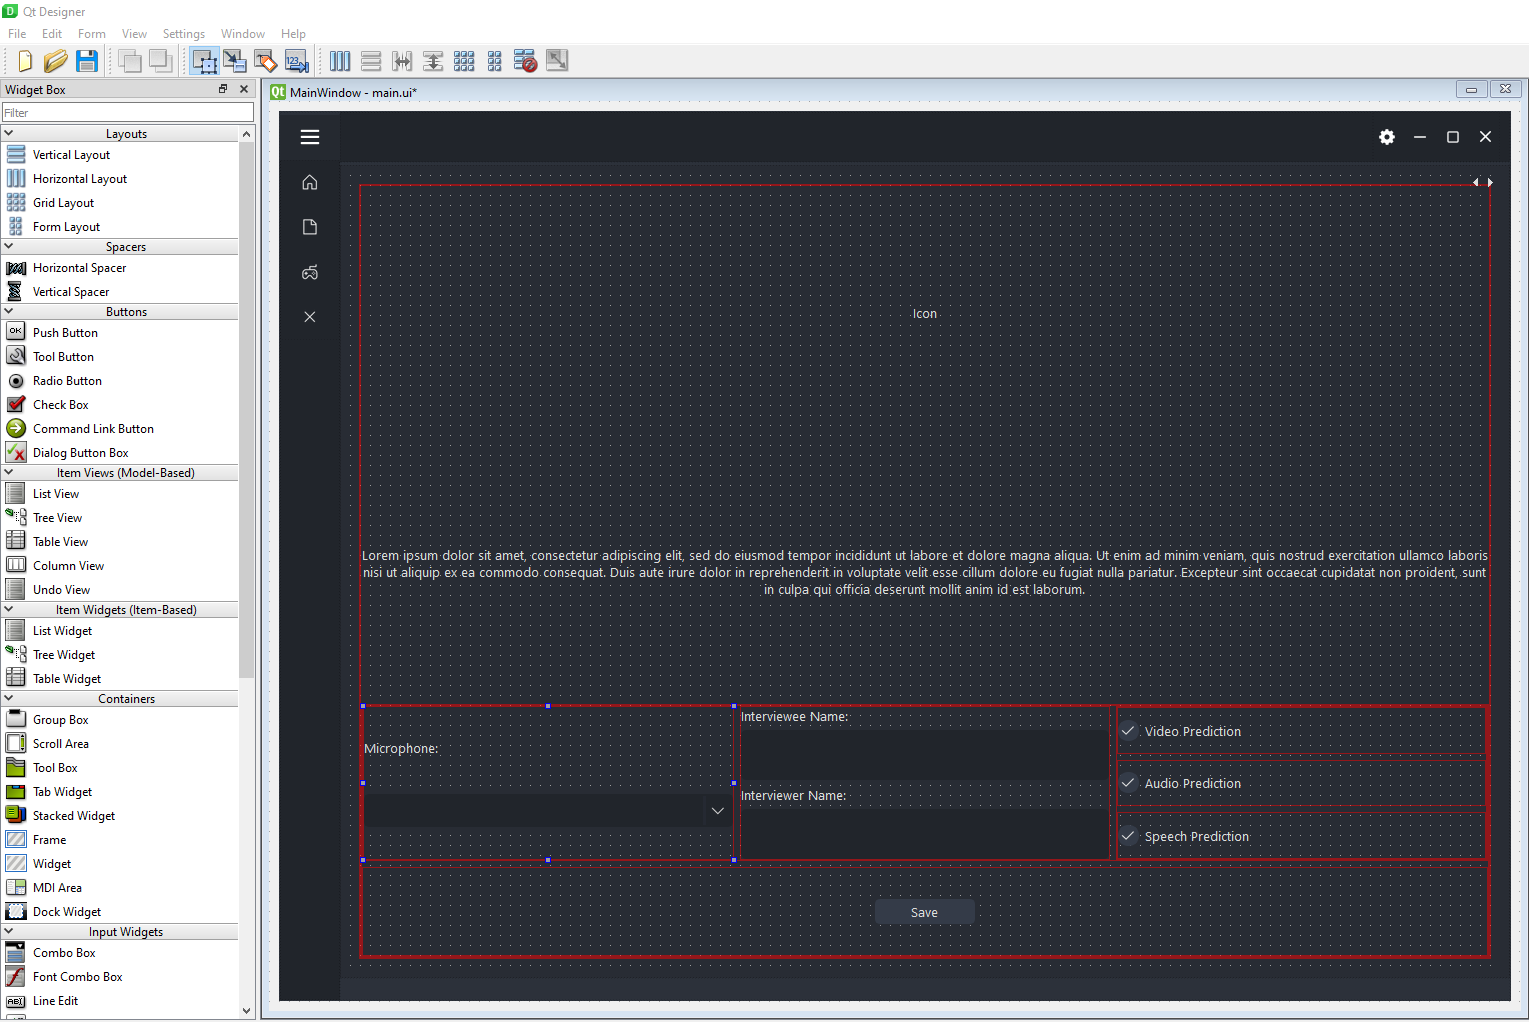
\includegraphics[scale=0.3]{images/qt_designer.png}
		\end{center}
		\caption{Qt Designer}
		\label{fig:qt_designer}
	\end{figure} 

	Printre principalele elemente utilizate preponderent în aplicație, le vom menționa pe următoarele (precum și informații referitoare la utilizarea lor în implementarea curentă):
	\begin{itemize}
		\item Aspect (layout): acest element este folositor atunci când se dorește organizarea elementelor copil după anumite reguli. Cele mai utilizate layout-uri sunt:
		\begin{itemize}
			\item Tip vertical: așezarea widget-urile copii va avea loc într-o manieră verticală, ca o stivă;
			\item Tip orizontal: constrânge ca widget-urile copil să fie așezate, în funcție de direcția aleasă, într-un mod longitudinal;
			\item Tip grilă: în funcție de dimensiunea aleasă, fiecare element copil utilizat în acest aspect va fi așezat într-un mod tabelar;
		\end{itemize}
		\item Elemente interactive:
		\begin{itemize}
			\item Buton: element de bază în aplicație, prin suprascrierea comportamentului unui buton, a fost posibilă interacționarea cu funcțiile aplicației (recunoașterea emoțiilor, suspendarea acestui proces sau oprirea);
			\item Casetă cu alegere: în general utilizat atunci când se dorește ca utilizatorul să aleagă între variante multiple;
			\item Casetă cu bifă: folositor pentru valori binare (adevărat sau fals). În cadrul aplicație, este utilizat pentru a permite utilizatorului să aleagă între funcționalitățile de recunoaștere pe care dorește să le utilizeze;
			\item Glisor: acest element ne va ajuta pentru derularea interviului salvat, în momentul în care se dorește vizualizarea lui;
			\item Zonă de text: utilizate pentru a oferi candidatului capacitatea de a-și introduce numele;
			\item Etichetă: diferite informații legate la starea aplicației;
			\item Tabel: folosit atunci când se dorește vizualizarea rapoartelor salvate.
		\end{itemize}
	\end{itemize}
	
	\subsubsection{MongoDb}
	Este o bază de date NoSql, în care documentele sunt salvate în formatul JSON. Această tehnologie a fost creată de DoubleClick în anul 2007 după ce au constatat că soluțiile actuale pentru persistarea datelor nu sunt suficient de scalabile și optime pentru cerințele lor, postarea de reclame. 
	
	Ierarhizarea datelor se face pe colecții, iar fiecare informație salvată într-o colecție este privită ca un document. Se pot construi diferite interogări pentru a solicita datele, asemănător bazelor de date relaționale.
	
	Fiind ușor de manevrat, flexibilă și scalabilă, MongoDb a oferit suport pentru persistarea datelor culese din cadrul unui interviu. Fiecare colecție salvată în această bază de date este denumită după candidatul căruia i se strâng date. Printre informații care se pot regăsi într-o colecție, menționăm: numele persoanei care intervievează, data începerii și sfârșitului interviului precum și durata acestuia. 
	
	Datorită constrângerii de memorie per document (8 MB), pentru stocarea datelor importante reținute din interviu, a fost nevoie de împărțirea datelor asemenea unui lanț. Fiecare bloc de date (binar), are o referință bidirecțională, fiind posibilă ca o agregare a acestor segmente să compună datele interviului. Vizualizarea informațiile este posibilă folosind MongoDb Compass, un explorator care face cu putință vizualizarea atât a colecțiilor cât și a conținutului unui document.
	
	\subsubsection{Biblioteci utilizate}
	Datorită alegerii făcute în materie de limbaj de programare, python oferă o gama largă de biblioteci și pachete care s-au dovedit folositoare pe parcursul dezvoltării aplicației. Printre acestea, vom menționa pe cele care au avut un impact semnificativ în perioada definirii proiectului: 
	
	\begin{itemize}
	 	\item Keras: este un API de deep learning open source, dezvoltat de Google pentru implementarea rețelelor neurale. Este scris în python și este utilizat pentru a facilita implementarea rețelelor neurale. Oferă o abstractizare de nivel înalt, făcând astfel ca acest pachet să fie prietenos cu utilizatorii. Keras permite comutarea între diferite baze, Tensorflow fiind cea care este utilizată în aplicație. Acest pachet ne oferă un mod de lucru mai intuitiv, care a fost folosit pentru definirea și antrenarea modelelor din aplicația Multimodal Emotion Detection.
	
		\item Tensorflow: constituite o bibliotecă open source, utilizată în calculul numeric, bazat pe flux de date. A fost dezvoltat inițial de Google Brain Team din cadrul organizației de cercetare Google Machine Intelligence pentru învățarea automată și cercetarea rețelelor neuronale profunde, dar sistemul este suficient de general pentru a fi aplicabil și într-o mare varietate de alte domenii. Tensorflow poate fi utilizat pe diverse procesoare: grafice, centrale și tensoriale. Folosit preponderent în aplicație, Tensorflow a fost utilizat pentru a face posibilă antrenarea modelelor neurale pentru fiecare perspectiva: audio, video și text.
	
		\item PyAudio: ne oferă suport pentru ascultarea, înregistrarea și salvarea fișierelor audio. Este definit cu un strat adițional pentru a permite apelarea metodelor din platforma PortAudio. Pachetul respectiv a oferit posibilitatea de a înregistra vocea candidatului în timpul interviului, precum și salvări de fișiere temporare, folosite în scopul analizei și a predicției emoției.
	
		\item Matplotlib: fiind o biblioteca cu utilizări în mai multe platforme, este folosit cu scopul vizualizării datelor grafice în python și extensia sa numerică numpy. Utilizarea acestui pachet în aplicație a fost împlinită prin afișarea datelor grafice precum: anvelopa acustică a unui fișier audio, spectogramele secvențelor de 4 secunde din date.
	
		\item OpenCv-Python: reprezintă un pachet de tipul API, care face posibilă utilizarea funcționalității din OpenCv prin apelarea metodelor scrise în C/C++. Acesta oferă suport pentru utilizarea camerei web, precum și diferite metode folosite în computer vision: calcularea de histograme, transformarea imaginilor în diferite canale (RGB, gri), modificare individuală a pixelilor, aplicarea de filtre. Prin utilizarea acestui pachet împreună cu Dlib, s-a putut realiza afișarea informațiilor referitoare la emoții în timp real, desenarea trăsăturilor feței (ochi, nas, gură etc).
	
		\item Librosa: este un pachet utilizat în special pentru analiza sunetelor. Permite funcționalități precum încărcarea/scrierea fișierelor audio în diferite extensii dar mai presus de menționat, aplicarea tehnicilor de procesare de semnal, precum transformata Fourier, spectograme în scala Mel etc.
	
		\item Pymongo: funcționează pe post de driver, făcând posibilă apelarea principalelor funcționalități ale MongodDb prin intermediul limbajului de programare python.
	\end{itemize}
	
	\subsubsection{Șabloane de proiectare}
	Șabloanele de proiectare au luat naștere din cauza problemelor de proiectare recurente și similare. Prin urmare, a devenit necesară conceptualizarea problemelor de proiectare în așa fel încât aceleași răspunsuri să fie refolosite de fiecare dată când apare o problemă similară.

	O problemă care s-a rezolvat utilizând șablonul "State Machine" este referitoare la administrarea ferestrelor precum și a navigabilității între acestea. Nu dorim ca utilizatorul să aibă șansa să comute între cadre atunci când este în timpul procesului de recunoaștere a emoțiilor. Astfel, mai jos sunt definite stările aplicației (\ref{fig:state}): acasă (meniul principal), recunoaștere, start recunoaștere, pauză recunoaștere, stop recunoaștere, rapoarte, vizualizare raport, ieșire.
	
	\begin{figure}[H]
		\begin{center}
			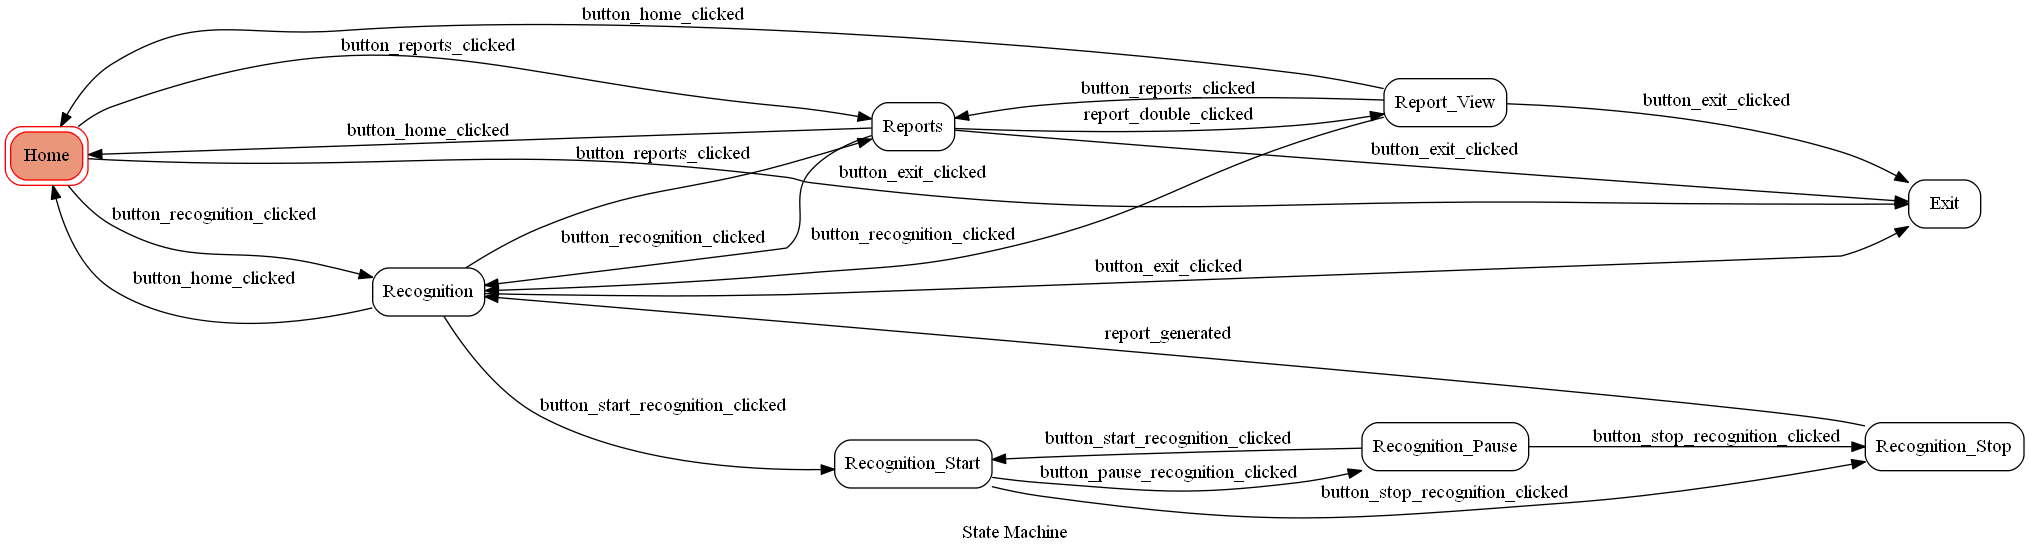
\includegraphics[scale=0.2]{images/state_diagram.png}
		\end{center}
		\caption{State machine aplicație}
		\label{fig:state}
	\end{figure} 	
	
	Pentru folosirea logging-ului, am ales utilizarea șablonului "Chain of Responsability". Acesta șablon funcționează după următorul principiu: dacă se întâmplă un eveniment care depășește capabilitățile de manevrare a obiectului în cauză, acesta va apela un superior, care va fi în stare să se ocupe de acest aspect. Logarea informațiilor este un proces important, deoarece printr-o analiză a datelor salvate, putem înțelege dacă s-a produs vreo malfuncție în timpul rulării. Șablonul are aplicabilitate în acest caz în momentul în care se produce o eroare. În funcție de severitatea erorilor, acestea vor fi manevrate de câte o clasa specială. 
	
	În aplicație, sunt definite o serie de clase care este suficientă doar o singură instanța. Utilizând "Singleton", putem forța crearea doar a unei instanțe, precum clasa care să aibă în vedere apelurile de CRUD în baza de date. 
	
	Având aceste informații, în următorul capitol vor fi prezentate cele două module definite în aplicație: recunoașterea emoțiilor în timp real și vizualizarea raportului.
	
	\clearpage
	\section{Aplicația Multimodal Emotion Detection}
	\subsection{Introducere}
	
	Multimodal Emotion Detection este o aplicație desktop, scrisă în limbajul de programare python, care utilizează tehnici de procesare de semnal, procesare de text și învățare automată cu scopul identificării emoțiilor umane, în contextul unui interviu. Principalele funcționalități ale acestei aplicații sunt reprezentate de:
	\begin{itemize}
	 	\item \textbf{Identificarea emoțiilor în timp real}: funcționalitate în care în timp real, sunt identificate emoțiile candidatului percepute din voce, expresii faciale precum și dialogul contextual recunoscut prin intermediul speech-to-text
		\item \textbf{Vizualizarea raportului}: după ce raportul interviului a fost generat, acesta poate fi vizualizat într-o fereastră dedicată
	\end{itemize}

	Când pornim aplicația, suntem întâmpinați de fereastra de introducere. Aceasta este construită dintr-o imagine de tip logo, o scurtă descriere a aplicației precum și o serie de setări, pe care utilizatorul le poate modifică după bunul plac.
	
	Aplicația oferă utilizatorului prilejul de a își introduce numele precum și alegerea dispozitivului audio pe care dorește să îl utilizeze pentru înregistrare. Mai mult decât atât, se poate activa/dezactiva fiecare funcționalitate majoră a aplicației (recunoaștere audio, video și text), în funcție de preferințele și modul de utilizare.
	
	Din acest moment, avem la dispoziție următoarele interacționări pe care le putem avea cu aplicația: recunoașterea emoțiilor în timp real sau vizualizarea rapoartelor.
	
	În cadrul recunoașterii emoțiilor în timp real, automatul de stare ne constrânge interacțiunea cu interfața grafică, pentru a nu crea probleme notabile în securitatea aplicației. Toate rapoartele asociate cu persoană intervievată vor fi încărcate în momentul în care se decide schimbarea numelui din setări. Dacă se dorește analiza unui raport generat în urma interviului, se va putea face într-un mod dedicat, unde se vor putea detecta informații esențiale și prețioase referitoare la emoțiile candidatului.
	
	\bigskip
	Pentru început, vom vorbi despre fiecare dintre funcționalitățile asociate primului modul, urmând mai apoi să fie prezentate aspecte referitoare interfeței grafice utilizate. Se vor detalia elementele de design grafic folosite în aplicație, precum și modul în care acestea ar trebui folosite. După prezentarea primului modul, se va începe o discuție referitoare la modulul de analizare a raportului, împreună cu funcționalitățile disponibile în acesta.
	
	\clearpage
	\subsection{Identificare emoțiilor în timp real}
	Fereastra pentru identificarea emoțiilor în timp real este alcătuită din 3 secțiuni (Figura \ref{fig:emotion_recog_clean}). Prima secțiunea este reprezentată de eticheta "Video", unde fluxul video va fi redat împreună cu predicțiile din expresia facială.
	
	\begin{figure}[H]
		\begin{center}
			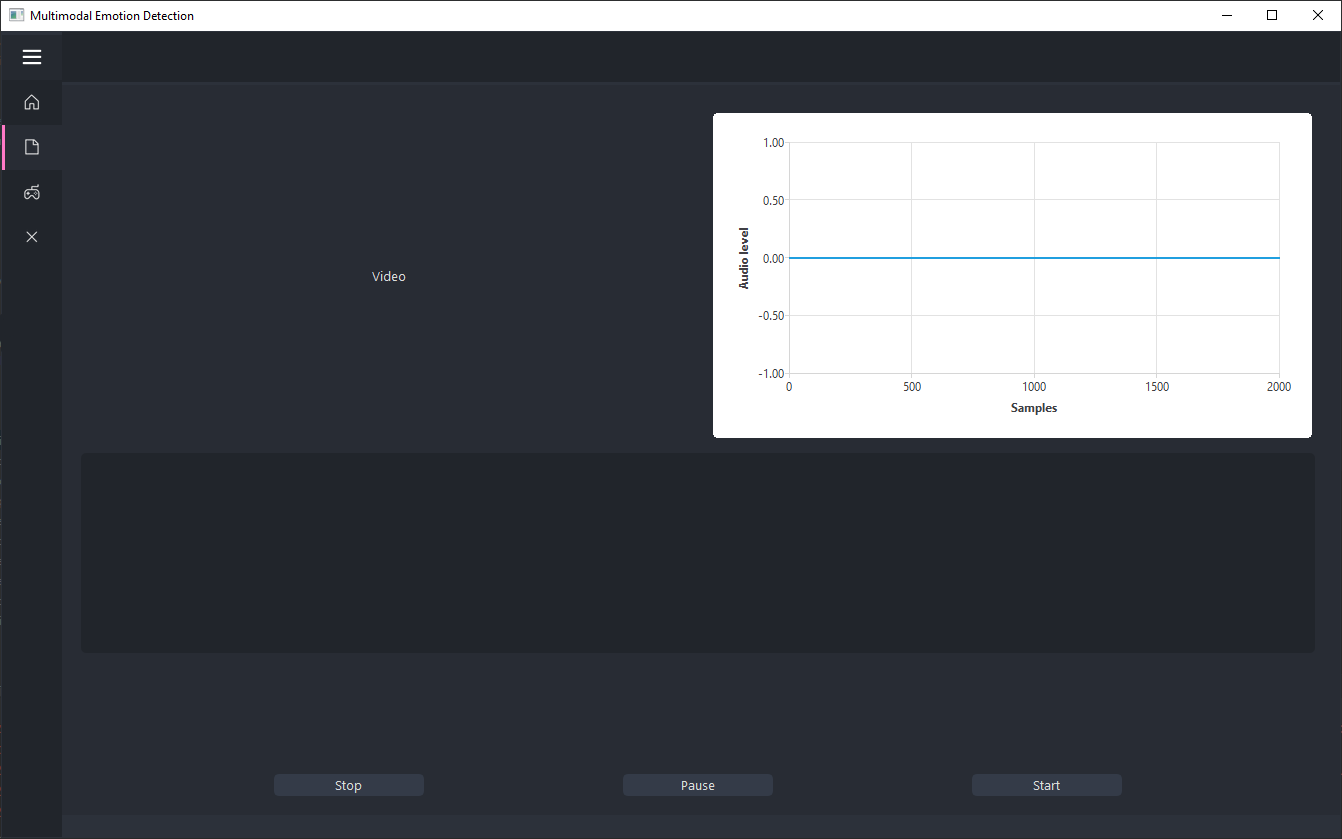
\includegraphics[scale=0.4]{images/emotion_recognition_clean.png}
		\end{center}
		\caption{Identificarea emoțiilor}
		\label{fig:emotion_recog_clean}
	\end{figure} 
	
	În partea din dreapta, se poate observa un grafic, în care acesta va fi actualizat conform cu impulsurilor din vocea candidatului. Microfonul se poate selecta, în funcție de cel dorit pentru a putea fi utilizat în identificarea emoțiilor. Mai jos, se poate observa o secțiune destinată afișajului de text. Utilizând tehnologia de speech-to-text oferită de Google, vom putea afișa dialogul avut de către candidat.
	
	Pentru ca aplicația să suporte predicția emoțiilor în timp real fără a bloca firul de execuție principal, este nevoia ca fiecare dintre cele 3 funcționalități să lucreze pe fir de execuție separat. În acest fel, interacționarea cu interfață grafică nu va fi blocată, iar utilizatorul va avea o experiență plăcută.
	
	Funcționalitățile de baza ale acestui modul sunt următoarele: recunoașterea emoțiilor audio, video și text.	
	
	\subsubsection{Recunoașterea emoțiilor audio}
	Ca un model inteligent de IA să fie capabil să identifice emoțiile umane din voce, este nevoie să fie antrenat pe un set de date specializat în acest context. Setul de date utilizat în identificarea stărilor din intermediul vocii este "Ryerson Audio-Visual Database of Emotional Speech and Song" (RAVDESS) \cite{ravdess}. Din acest set de date au fost utilizate doar fișierele audio.

	Fișierele audio selectate pentru antrenare sunt caracterizate de 16 bit-depth și rată de eșantionare 48 kHz. Sunt în număr de 1440 fișiere: 60 de înregistrări per actori x 24 de actori. Au fost angajați 24 de interpretori profesioniști (12 de sex masculin, 12 sex feminin), care vocalizează două afirmații lexicale într-un accent neutru nord-american. Emoțiile pe care actorii le reproduc sunt următoarele: neutru, fericire, tristețe, furie, teamă, surprindere și dezgust, unde adițional este adăugat o intensitate emoțională (normală și puternică).

	Fiecare din cele 1440 de fișiere au un nume unic. Numele unui fișier constă dintr-un identificator numeric construit din 7 părți (03-01-06-01-02-01-12.wav), în extensie wav. Acești identificatori definesc caracteristicile stimulului:
	
	\begin{itemize}
		\item Modalitatea: 01 = audio-video, 02 = video, 03 = audio;
		\item Interpretare: 01 = vorbit, 02 = cântat;
		\item Emoție: 01 = neutru, 02 = calm, 03 = fericit, 04 = trist, 05 = furios, 06 = teamă, 07 = dezgust, 08 = surprins;
		\item Intensitate emoțională: 01 = normal, 02 = puternic;
		\item Propoziția rostită: 01 = "Kids are talking by the door", 02 = "Dogs are sitting by the door";
		\item Numarul de repetări: 01 = o repetare, 02 = două repetări;
		\item Identificatorul actorului: de la 01 la 23; actorii cu număr impar sunt barbați iar cei cu număr par femei.
	\end{itemize}

	Motivația din spatele alegerii acestui set de date este susținută de calitatea înaltă a vocilor înregistrate, cât și performanțele ridicate ale actorilor care interpretează propozițiile.
	
	În Figura \ref{fig:audio_plot} este reprezentat un fișier audio într-o manieră grafică. În procesul de preprocesare al datelor, a fost nevoie de o normalizare a lor. Deoarece unele fișiere nu erau de aceeași dimensiune, în procesul de normalizare a fost nevoie să se trunchieze sau să extrapolăam date până când toate acestea să aibă dimensiunea de 48000.
	
	\begin{figure}[H]
		\begin{center}
			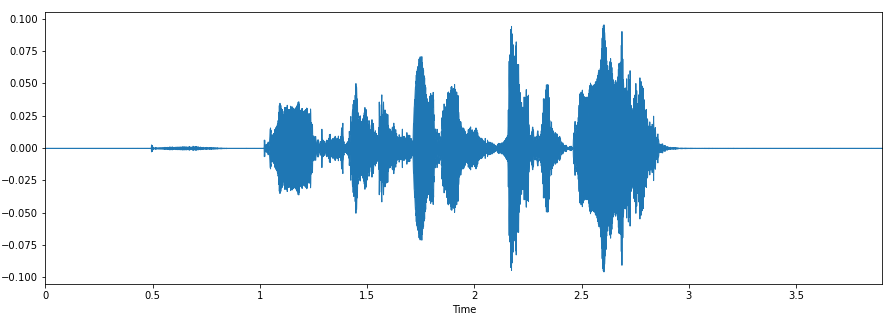
\includegraphics[scale=0.6]{images/audio_plot.png}
		\end{center}
		\caption{Fișier audio reprezentat grafic}
		\label{fig:audio_plot}
	\end{figure}
	
	Adițional, a fost utilizat z-score (standard score), o tehnică care indică la câte deviații standard se află datele față de medie. Scopul aplicării acestei normalizări este de a sporii eficientă rețelei neurale în faza antrenării. Mai mult decât atât, pentru a reduce riscul de overfitting al modelului, a fost creată o copie, peste care s-a adăugat un semnal de tipul sinus. Teoretic, se va adaugă un zgomot de fundal, scăzând șansele modelului a se specializa în profunzime pe aceste date.
	
	După pasul de preprocesare, este nevoie ca din datele să fie extrase caracteristicile esențiale pe care dorim ca modelul să le învețe. Deoarece în domeniul frecvențelor putem găsi mai multe informații, utilizând STFT, fiecare fișier audio va fi adus în această gamă. Rezultatul obținut prin aplicarea acestei tehnici va reprezenta o spectrogramă simplă, care nu este îndeajuns pentru a putea face o distincție corectă dintre emoțiile vocii umane. 
	
	Problema reiese din cauza modului în care urechea umană este construită. Urechea umană este de așa natură încât să poată distinge foarte ușor schimbările semnalelor acustice emise la frecvențe joase față de cele înalte. Altfel spus, vom putea distinge cu ușurință sunetele care au o frecvență joasă (spre exemplu, un robinet deschis are o frecvență de aproximativ 250 Hz) față de cele înalte (un fluier cu ultrasunete folosit în dresajul câinilor, având o frecvență cuprinsă între 2000 și 25000 Hz). Practic modul în care urechea umană percepe sunetul este asemănător cu funcția logaritm.
	
	Pentru a putea converti în scala Mel putem utiliza formula de mai jos :
	\begin{equation}
	\label{to_mel_scale}
		m=1125 * ln(1+f/700)
	\end{equation}
	
	Aplicând formula \ref{to_mel_scale}, spectrograma inițial creată este transformată în spațiul Mel, domeniu care se aseamănă mai mult cu modul in care urechea umană percepe sunetul.
	
	Având acest rezultat intermediar, pentru o acuratețe mai mare a modelului, următorul pas în procesul de preprocesare a fost segmentarea în unități egale intercalate. Acest pas este susținut de sporirea eficacității modelului precum și de creșterea granularității datelor.
	
	\begin{figure}[H]
		\begin{center}
			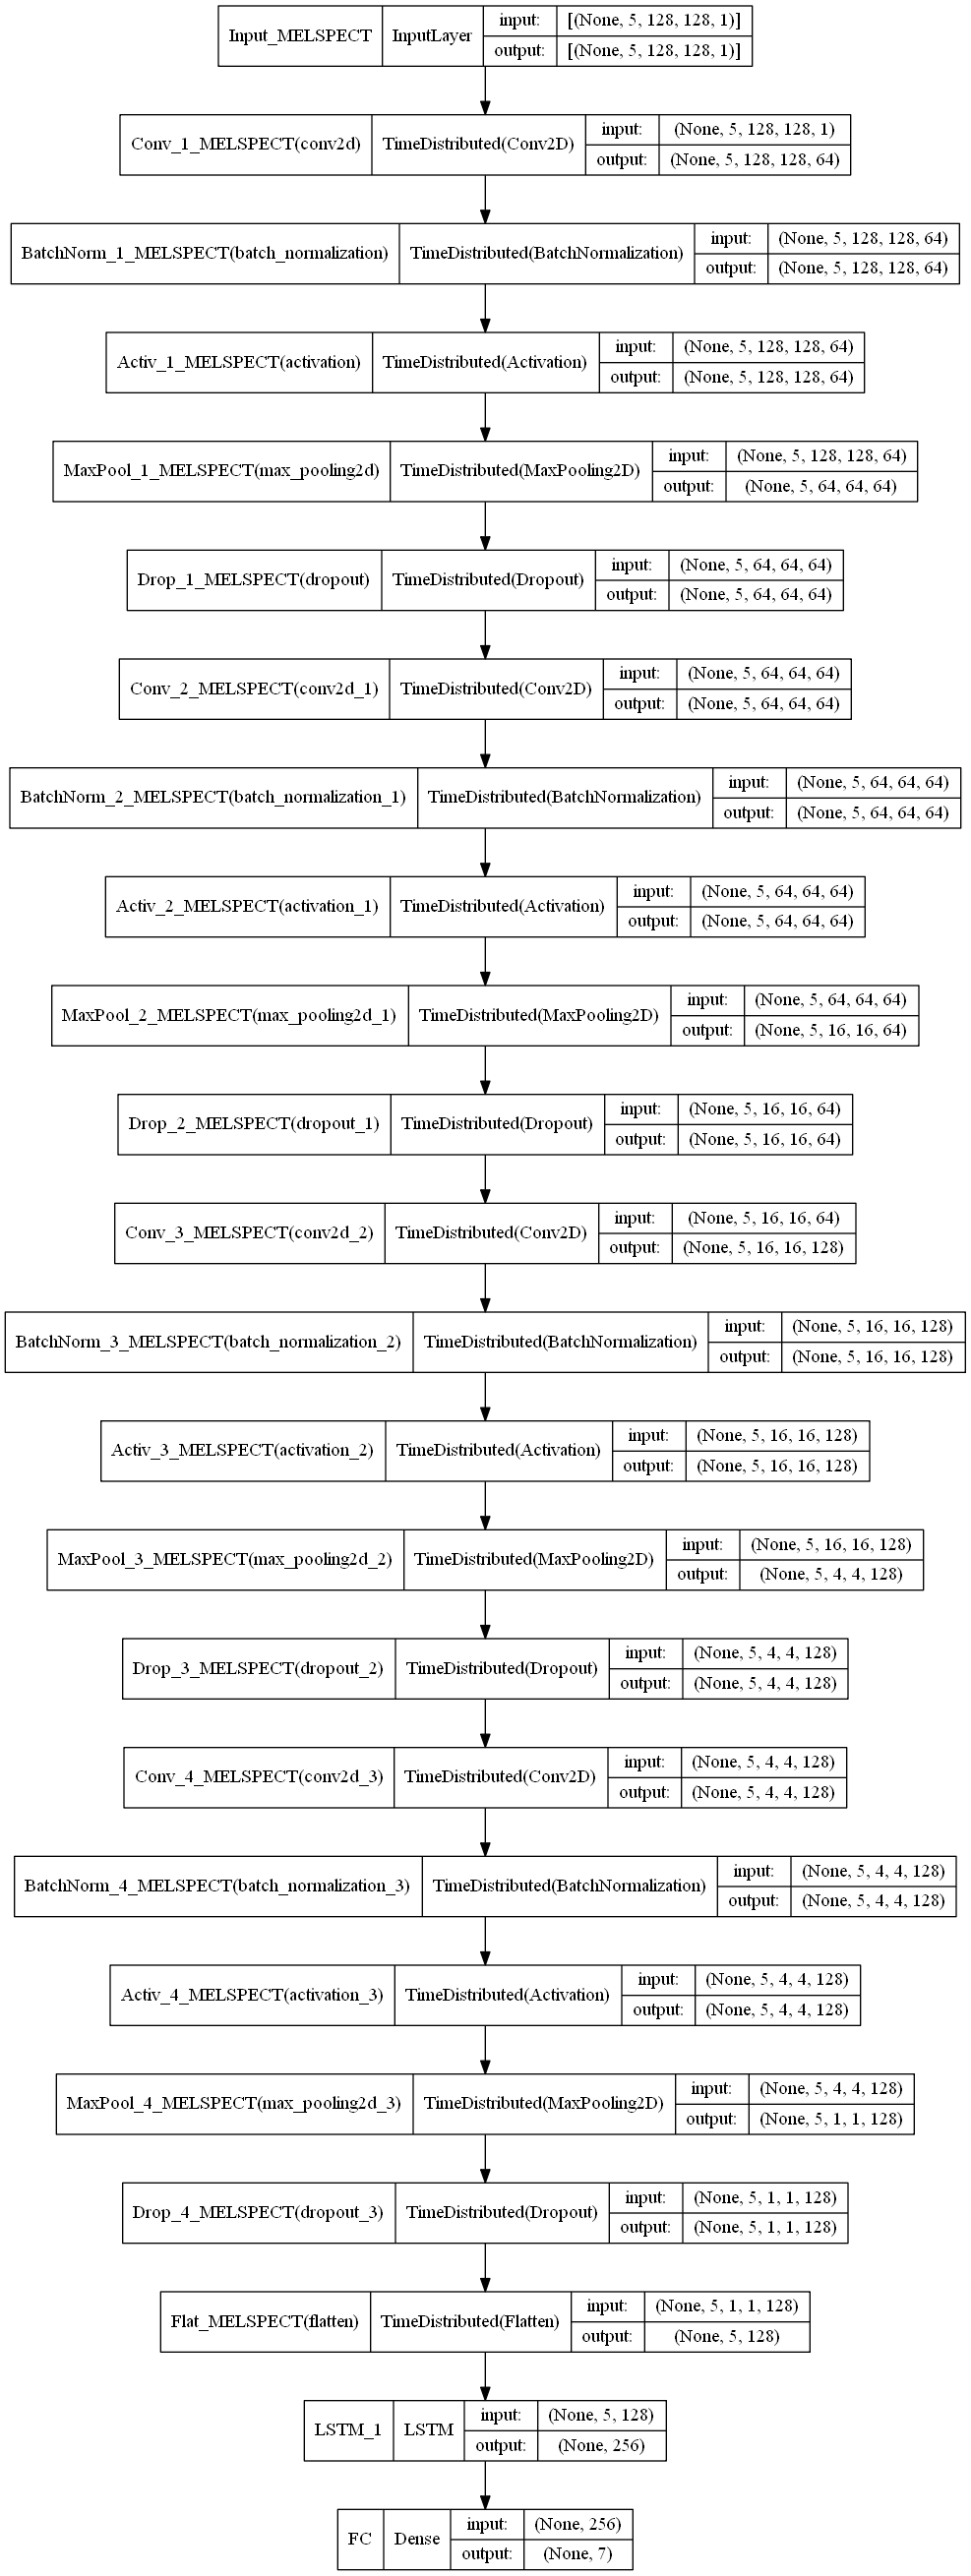
\includegraphics[scale=0.2]{images/audio_model.png}
		\end{center}
		\caption{Arhitectura modelului de predicție audio}
		\label{fig:audio_model}
	\end{figure}
	
 	În Figura \ref{fig:audio_model} se poate observa arhitectura modelului utilizat pentru predicțiile audio. Este construit din straturi convolutionale, cu număr de filtre variabil (64 sau 128). Pentru stabilizarea procesului de învățare și reducerea drastică a numărului de epoci de antrenament necesare antrenării rețelei, au fost utilizate straturile care să normalizeze batch-urile. Pentru reducerea spațială a parametrilor utilizați în calcule și pentru evitarea overfitting-ului, după fiecare strat convoluțional, a fost adăugat un strat max pooling. Funcția de activare folosită preponderent în acest model este Exponential Linear Unit. 
 	
 	Mai mult decât atât, fiecare strat menționat mai sus a fost învelit într-un strat de timpul long short-term memory, eficient de utilizat în cazul predicțiilor în care datele sunt de tipul secvență. Datorită preprocesării anterioare și a împărțirii pe segmente intercalate, acest strat s-a dovedit util de folosit, datorită proprietății de stocare internă a memoriei.
	
	\begin{figure}[H]
		\begin{center}
			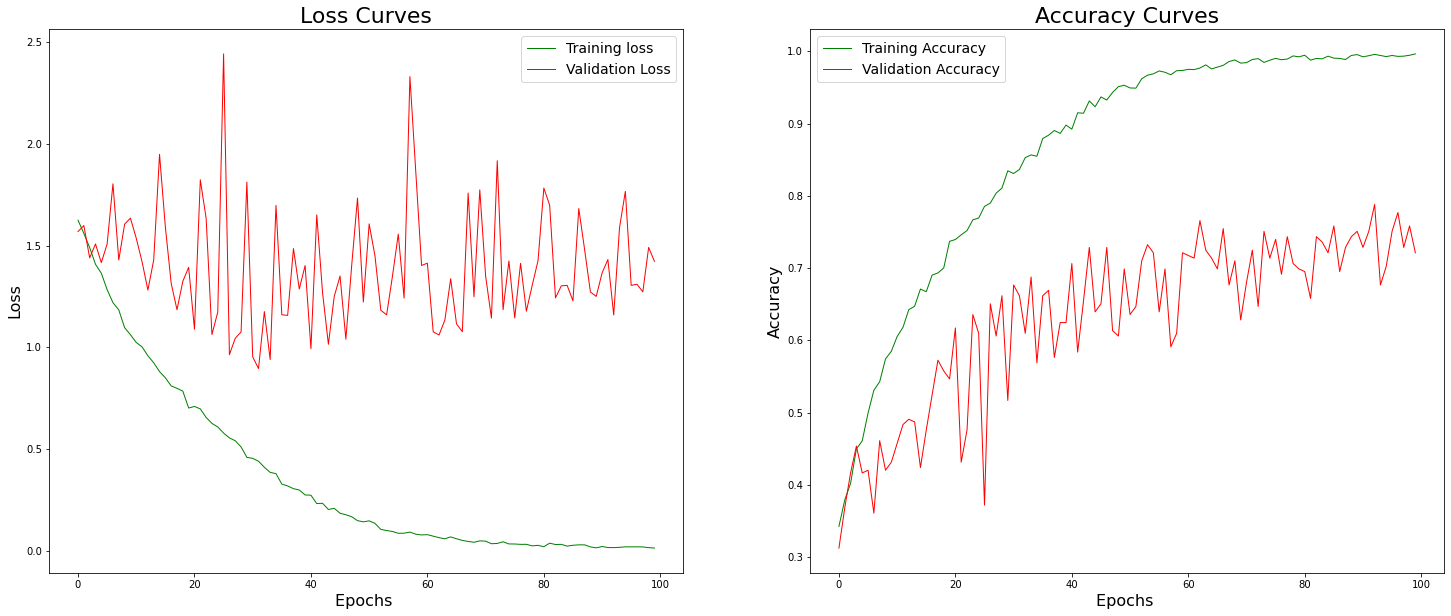
\includegraphics[scale=0.2]{images/accuracy_audio_model.png}
		\end{center}
		\caption{Statistici model audio}
		\label{fig:audio_model_accuracy}
	\end{figure}
	
	Acuratețea înregistrată pe datele de testare este una ridicată, aproximativ 95.91\%. În Figura \ref{fig:audio_model_accuracy} se poate observa procesul de învățare al modelului, precum și plafonarea pe care acesta o are la final, datorită numărul de epoci și batch-uri executate.
	
	\begin{figure}[H]
		\begin{center}
			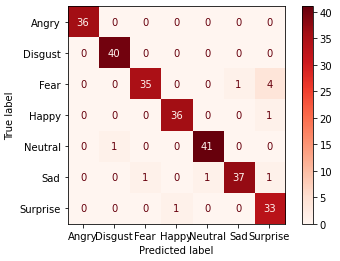
\includegraphics[scale=0.7]{images/audio_confusion_matrix.png}
		\end{center}
		\caption{Matrice de confuzie model audio}
		\label{fig:audio_confusion_matrix}
	\end{figure}

	Prin Figura \ref{fig:audio_confusion_matrix} se observă matricea de confuzie asociată predicțiilor pe datele de testare. Se poate observa cum modelul a făcut confuzie între starea de frică și cea de surprinde, care pot fi destul de asemănătoare din punct de vedere vocal.
	
	%In cadrul acestei persepective, emotiile sunt transmise prin intermediul vocii. Analizand aproximativ 4 secunde de date la rata de esantionare de 16 kHz, se vor aduna suficiente date pentru a se putea face o predictie in timp real.
	
	\clearpage
	\subsubsection{Recunoașterea emoțiilor video}
	Pentru identificarea stărilor și emoțiilor din expresiile faciale, a fost nevoie de conceperea unui set de pași:
	\begin{itemize}
		\item Detectarea facială.
				
		Pentru acest pas al algoritmului creat, Dlib ne pune la dispoziție două rețele prin care se pot identifica fețe umane. Este vorba despre: HOG + Linear SVM și Max-Margin (MMOD) CNN. Prima tehnică este mai eficientă și mai rapidă, dar nu la fel de precisă cum este a două. În aplicație, s-a făcut un compromis pentru a avea performanțe mai ridicate, utilizând prima rețea de recunoaștere. 
		
		\item Identificarea marginilor zonei faciale.
		
		Ca rezultat în urmă identificării faciale, acesta va fi reprezentat de către coordonatele XOY ale dreptunghiului în care față umană a fost identificată.
		
		\begin{figure}[H]
			\begin{subfigure}[b]{0.5\textwidth}
				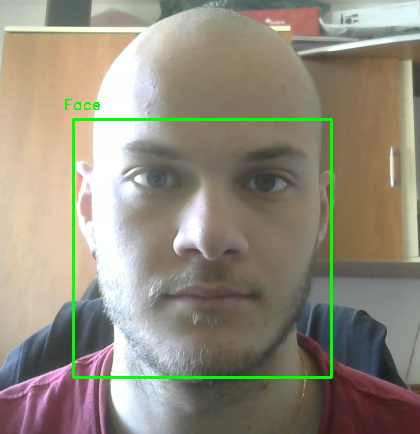
\includegraphics[width=\textwidth]{images/face_detected.png}
				\caption{Detectarea feței}
				\label{fig:video_face_detection}
			\end{subfigure}
			\hfill
			\begin{subfigure}[b]{0.425\textwidth}
				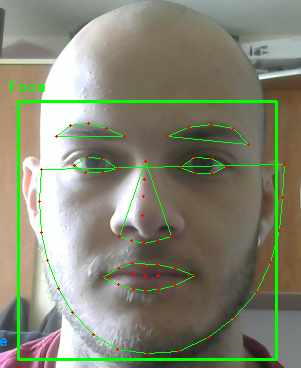
\includegraphics[width=\textwidth]{images/face_features.png}
				\caption{Denesarea trăsăturilor faciale}
				\label{fig:video_face_features}
			\end{subfigure}
			\caption{Plotarea feței}
			\label{fig:face}
		\end{figure}
	
		Prin intermediul pachetului OpenCv, putem trasa mai departe diferite forme geometrice (exemplu Figura \ref{fig:video_face_detection}) care să evidențieze zona de interes.
		
		\item Decuparea feței.
		
		Deoarece mai departe este nevoie de strict de zona feței pentru a se putea face predicția referitor la emoțiile candidatului, aceasta va fi salvată separat pentru a putea fi procesată. 
		
		\item Evidențierea trăsăturilor feței.
		
		Pentru a putea oferi o interfață mai prietenoasă utilizatorului, sunt evidențiate următoarele trăsături ale feței: sprâncene, ochi, nas, gură și conturul maxilarului (Figura \ref{fig:video_face_features}). 
		
		\item Transformarea în nuanțe de gri.
		
		Pentru că în setul de date utilizat, datele sunt în grey-scale, nu a mai fost necesar să facem această transformare. Motivația din spate este dată de eficientizarea calculelor, fiind suficient ca operațiile matematice să fie efectuat pe singurul canal disponibil, gri.
		
		\item Predicția zonei de interes.
		
		Având acest rezultat intermediar, datele aferente feței vor fi procesate mai apoi de către modelul de IA folosit pentru predicția emoțiilor din expresiile faciale.
		
	\end{itemize}
	
	Datele utilizate pentru antrenare rețelei artificiale provin din setul de date "Facial Emotion Recognition" (FER 2013). Datele constau din imagini de 48x48 pixeli în tonuri de gri ale fețelor, fiind în număr de 28709 poze. Fețele au fost înregistrate automat, astfel încât fața să fie mai mult sau mai puțin centrată și să ocupe aproximativ aceeași cantitate de spațiu în fiecare imagine. Categoriile de emoții sunt: 0 = Furios, 1 = Dezgust, 2 = Frică, 3 = Fericit, 4 = Trist, 5 = Surprins, 6 = Neutru.
	
	Informațiile sunt reținute în format csv, având două coloane: emoție și pixeli. Pe coloana emoție, conține un număr de la 0 la 6 pentru emoția reprezentată în imagine. Coloana pixeli conține un șir de numere între ghilimele pentru fiecare imagine. Conținutul acestui șir are valori de pixeli separate de spațiu în ordinea majoră a rândurilor. În Figura \ref{fig:video_dataset_example}, este printată un exemplu din setul de date.
	
	\begin{figure}[H]
		\begin{center} 
			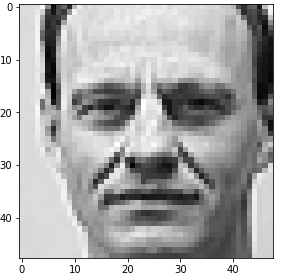
\includegraphics[scale=0.7]{images/video_dataset_example.png}
		\end{center}
		\caption{Canditat set de date video}
		\label{fig:video_dataset_example}
	\end{figure}
	
	În etapa de preprocesare, a fost urmată o structură mai ușoară. Deoarece datele erau deja în tonuri gri, ultimul pas care trebuia aplicat era cel de normalizare al datelor. Astfel, datele care reprezintă pixelii (intensitatea de gri), au fost normalizate între 0 și 1, pentru a spori performanțele în timpul antrenării modelului.
	
	Arhitectură utilizată pentru modelul de învățare video este inspirată din model Xception \cite{xception}, creat chiar de fondatorul pachetului Keras. Modelul este construit astfel, în 3 etape: fluxul de intratre, mijloc și final. Fiecare dintre aceste nivele se bazează pe perechi de straturi convolutional separabil, normalizare și activare. 
	
	Pentru a elimina riscul de overfiting, se utilizează un generator sintetic de date, care are rolul a crea date destul de asemănătoare celor date, adăugând următoarele operații asupra lor: mărirea, rotirea, mutarea ei în cele patru direcții cardinale precum și întoarcerea ei pe orizontală și verticală. În acest sens, minimizăm pe cât posibil riscul de overfitting al modelului pe datele de antrenare.
	
	În scop de testare, prin izolarea a primelor straturi din rețea, am putut observa modul în care rețeaua neurală își creează hărți de caracteristici pe baza unei poze date. Este de reținut că în acest pas, rețeaua nu este antrenată, caracteristicile găsite putând să fie schimbate de la o epocă la altă.
	
	\begin{figure}
		\centering
		\begin{subfigure}[b]{0.8\textwidth}
			 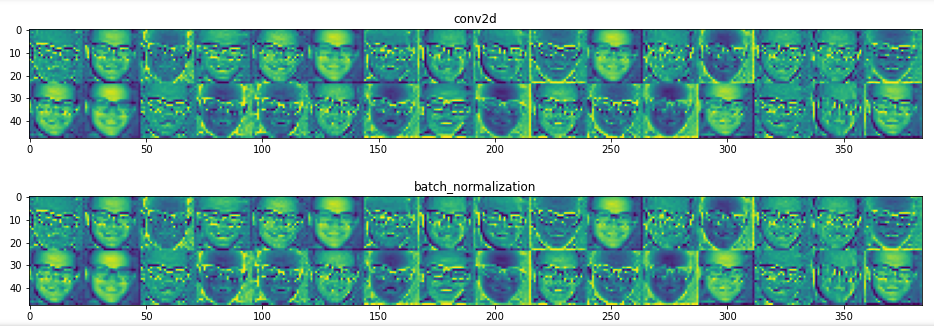
\includegraphics[width=1\linewidth]{images/video_model_layers_visualisation.png}
			\caption{Caracteristici primele straturi}
			\label{fig:video_model_layers_visualisation}
		\end{subfigure}
		\begin{subfigure}[b]{0.4\textwidth}
			 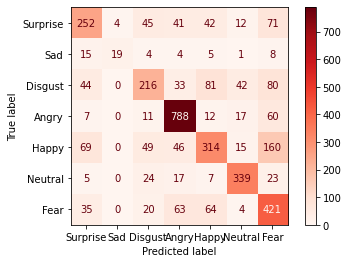
\includegraphics[width=1\linewidth]{images/video_confusion_matrix.png}
			\caption{Matrice de confuzie model video}
			\label{fig:video_confusion_matrix}
		\end{subfigure}
	\end{figure}

	În Figura \ref{fig:video_model_layers_visualisation} se poate observa că, în urma unei procesări care a permis vizualizarea datelor într-o formă mai lizibilă, imaginea dată pentru predicție este descompusă și analizată de rețea.

	Din punct de vedere al acurateței, acestă rețea are performanțe bune pentru acest set de date, având o precizie de 93.46\% pentru setul de validare, iar cazul setului de testare,  65.45\%. Se poate observa în Figura \ref{fig:video_confusion_matrix} performanțele modelului video din prisma matricei de confuzie.
	
	\clearpage
	\subsubsection{Recunoașterea emoțiilor din text}
	În cadrul detectării emoțiilor din text, setul de date utilizat se bazează pe rezultatul obținut din studiul "Linguistic styles: Language use aș an individual difference" \cite{text_dataset}. În realizarea acestui articol, au fost înregistrate 15 jurnale ale unor pacienți internați pentru abuz de substanțe, sarcinile zilnice ale a 35 de studenți și rezumatele jurnalelor a 40 de psihologi sociali. Obiectivul acestui studiu a fost acela de a demonstra că, limbajul pe care îl avem când scriem ne poate reflecta personalitatea.

	Din acest set date, au fost utilizate 2468 de articole scrise ale celor 35 de studenți. Din cele 35 de persoane care au participat la studiu, au fost 29 de femei și 5 bărbați, cu vârste cuprinse între 18 și 67 ani, media vârstei fiind de 27. Articolele folosite ca date, au fost sub forma unor sarcini fără evaluare. 

	Pentru fiecare temă, studenții trebuiau să scrie minim 20 de minute pe zi despre un anumit subiect. Datele au fost colectate în timpul unui curs de vară de 2 săptămâni între 1993 și 1996. Fiecare student și-a completat proba scrisă zilnic timp de 10 zile consecutive. 

	Scorurile de personalitate ale studenților au fost evaluate prin completarea chestionarului Big Five Inventory (BFI). BFI este un chestionar alcătuit din 44 de itemi care oferă un scor pentru fiecare din cele 5 trăsături de personalitate (OCEAN). O intrare din setul de date utilizat este construit din următorul format: 
	\begin{itemize}
		\item Id: identificatorul unic al fiecărui articol
		\item Text: este scris în limba engleză, și în mare parte, fiecare student își exprimă gândurile, starea și acțiunile pe care le-a făcut în ziua respectivă
		\item Cele 5 categorii de personalitate: pentru fiecare eticheta utilizată, i-a fost acordat "da", fie "nu", pentru a indica un punctaj ridicat sau scăzut pentru o anumită trăsătură.
	\end{itemize}

	Urmează un fragment folosit în setul de date: "Well, right now I just woke up from a mid-day nap. It is sort of weird, but ever since I moved to Texas, I have had problems concentrating on things. I remember starting my homework in 10th grade as soon as the clock struck 4 and not stopping until it was done. Of course it was easier, but I still did it."
	
	Este important de remarcat faptul că etichetele de clasificare au fost aplicate în funcție de răspunsurile la un chestionar destul de scurt. Datele pot fi "biased" sau nu atât de veridice precum am bănui, datorită autoevaluării studenților printr-un set de întrebări scurte. Ce se dorește să se remarce în acest paragraf este faptul că emoțiile și personalitățile umane sunt complexe.
	
	Preprocesarea datelor pentru a fi analizate în contextul detectării emoțiilor trebuie să fie una amănunțită. S-a urmat astfel, următorul set de pași:
	\begin{itemize}
		\item Eliminarea caracterelor non alfa-numerice, curățarea textului de diferite prepoziții și/sau prescurtări utilizând regex.
		\item Tokenizarea textului în propoziții, urmând mai apoi ca pentru fiecare să se aplice următoare operații:
		\item Împărțirea propoziției în cuvinte, determinând ce parte a propoziției este fiecare cuvânt (subiect, verb, adjectiv etc).
		\item Eliminarea cuvintelor de oprire și procesarea celor care trec mai departe de acest filtru prin reducerea cuvintelor la minusculă.
		\item Aducerea cuvintelor în formă lor inițială utilizând procesul de lematizare din WordNet. Se folosește acest procedeu în loc de alegerea rădăcinii cuvântului pentru a aduce la o formă mai apropiată în contextul dat.
		\item Vectorizare, prin transformarea perechilor identificate în numere
	\end{itemize}
	
	\bigskip
	
 	Rețeaua neurală antrenată utilizând acest set de date este construită din straturi de tipul: embedding, conv1d, maxpooling1d, batchNormalization și LSTM.

	Pentru a putea lucra cu date de tip text, trebuie ca datele lexicale să fie transformate în numere. Pentru rețele care se ocupă cu predicția pe diferite clase, se poate utiliza one hot encoding. Dar pentru cuvinte, această tehnică ne poate îngreuna procesul de învățare datorită șirurile mari de 0 și 1 care s-ar crea. O tehnică mai eficientă este reprezentată de utilizarea straturilor embedding, care vor ajuta la reprezentarea cuvintelor prin numere întregi. Stratul convolutional 1d este asemănător cu cel utilizat în cadrul imaginilor, singură diferența fiind între numărul de dimensiuni în care se face glisarea filtrelor.

	Predicția pentru identificarea personalității pe baza interviului va avea loc la final, deoarece sunt nevoie de cât mai multe date pentru a avea o acuratețe ridicată.
	
	\clearpage
	\subsection{Utilizare modul identificare emoții}
	Pentru a putea începe recunoașterea emoțiilor în timp real, suntem nevoiți să comutăm pe fereastra de identificare a emoțiilor. Înainte de a apasă pe butonul start, vom fi întâmpinați de o fereastră asemănătoare cu Figura \ref{fig:emotion_recog_clean}. Această fereastră este una curată, nefiind trecută prin procesul de intervievare. 

	După ce începem procesul de identificare a emoțiilor în timp real, în funcție de dispozitivele hardware disponibile (microfon, camera-web), aceasta vor înregistra datele necesare și le vom putea vizualiza în cele două panouri superioare.
	
	\begin{figure}[H]
		\begin{center}
			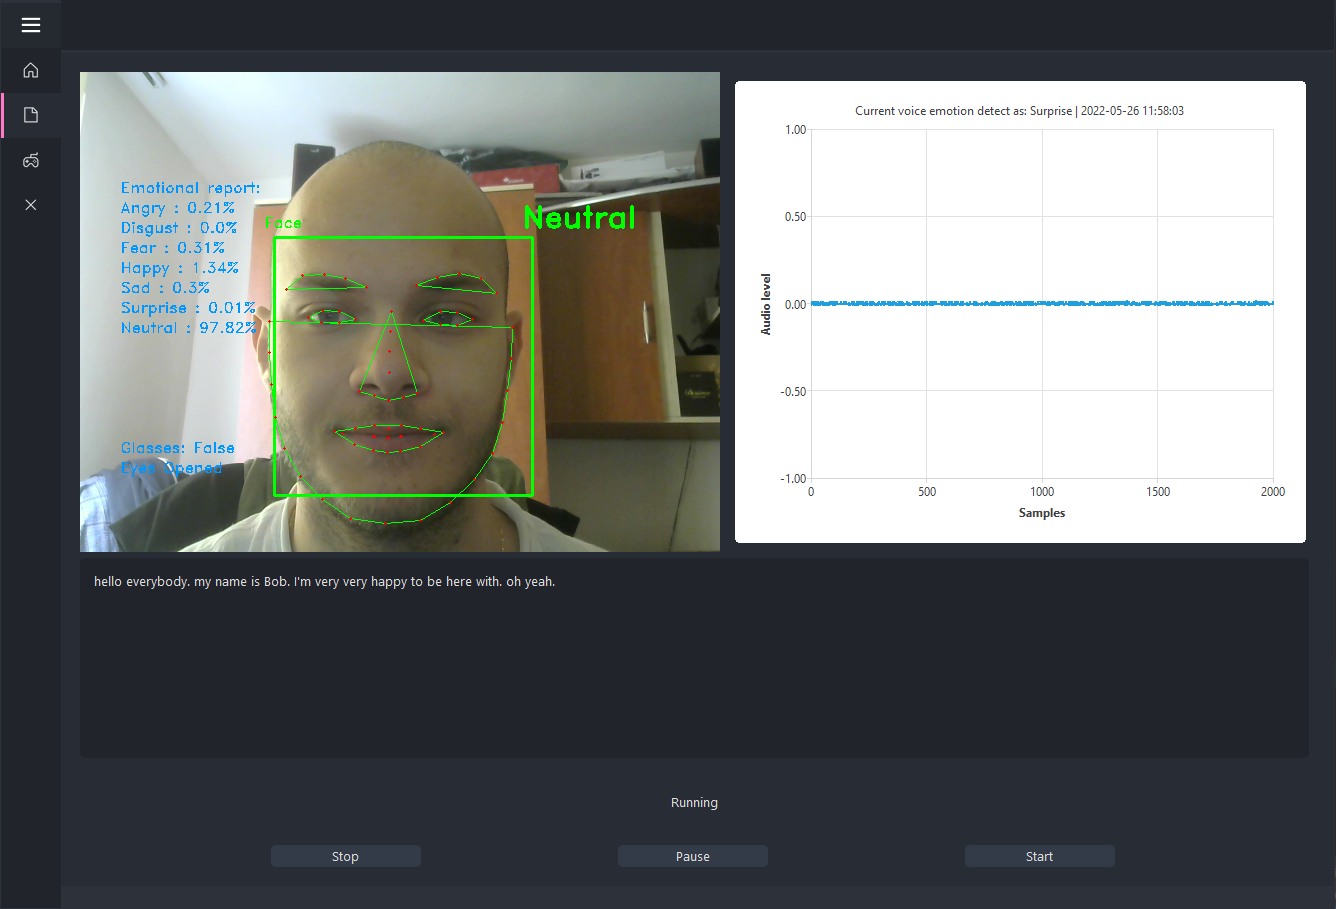
\includegraphics[scale=0.35]{images/emotion_recognition.png}
		\end{center}
		\caption{Identificarea emoțiilor în timp real}
		\label{fig:emotion_recog}
	\end{figure} 

	În Figura \ref{fig:emotion_recog}, este prezentată fereastra activă, în care se fac recunoașterile emoțiilor în timp real. În panoul situat în stânga, dedicat fluxului video, sunt afișate datele captate de camera web împreună cu procesarea live făcută de rețeaua neurală pentru predicția imaginilor. În partea stânga a imaginii, sunt afișate probabilitățile aferente fiecărei clase, precum și emoția expresiei faciale identificată. 

	În partea opusă, este prezentat un grafic, care afișează impulsurile audio captate de microfon. Inițial este precizat numele microfonului utilizat, urmând mai apoi să fie afișat emoțiile identificate. Inferior față de cele două zone discutate, se află un chenar în care textul recunoscut din dialogul candidatului este interpretat în cuvinte și atașat.

	Datorită restricțiilor impuse de către automatul de stare, în timpul recunoașterii emoțiilor, avem două acțiuni accesibile de către utilizator. Poate să pună pe pauză, mod în care determinarea emoțiilor este oprită sau poate să oprească definitiv acest proces, care va determina generarea raportului. Pe parcursul interviului, se poate vedea starea curentă a aplicației (Running, Paused, Stopped).

	\subsubsection{Generarera raportului}
	Pentru ca procesul de identificare a emoțiilor să fie în timp real, fiecare funcționalitate de recunoaștere este pornită într-un fir de execuția separat. Acest proces facilitează atât interfață grafică de a fi receptivă cu utilizatorul. Setul de date utilizat pentru antrenarea audio este construit din fișiere cu aproximativ lungime de 4 secunde. Având această constrângere, când firul care execută recunoașterea audio va înregistra 4 secunde de date, se va face o predicție, care va fi afișată și mai apoi, depozitată într-o clasă care colectează aceste date. 

	În cazul predicției video, în funcție de performanțele camerei (camera utilizată poate să acumuleze aproximativ 20 cadre pe secundă), cadrele sunt procesate, iar informațiile aferente afișate către utilizator, împreună cu rata de încredere a modelului pentru fiecare clasă. Pentru a reține doar cele mai reprezentative cadre necesare vizualizării raportului, la fiecare 4 secunde se alege acel cadru care cu cea mai proeminentă predicție și rată de încredere.

	Textul identificat din conversația candidatului este procesat, urmând mai apoi să fie transmis către clasa care se ocupă cu gestionarea datelor. 	

	Odată ce s-a oprit recunoașterea în timp real, iar atât datele audio, video și text au fost colectate, urmează generarea raportului. Cu ajutorul datelor colectate, se va crea o structură în care datele salvate și predicțiile vor fi persistate. Pentru a oferi oportunitatea ca interviul să fie revizuit, este necesar ca datele să fie salvate. Utilizând baza de date non-relațională MongoDb, am reușit să obținem persistarea datelor la nivel local.

	MongoDb având limitarea pentru mărimea colecțiilor (8 MB), datele care reprezintă cadrele foto, cât și segmentele audio în care s-au făcut predicțiile sunt stocate într-un mod binar, fiind înlănțuite pentru a putea face o reconstrucție într-un mod eficient. În momentul în care se dorește vizualizarea datelor, în funcție de numele introdus al candidatului, vor fi aduse datele aferente interviurilor lui. În cazul în care nu se introduce niciun nume, rapoartele vor fi salvate sub denumirea de "No Name".
	% diacritice
	\clearpage
	\subsection{Vizulizarea tuturor rapoartelor}
	După generarea raportului, din Figura \ref{fig:state}, se poate observă că vom reveni într-o stare, care ne permite navigarea către fereastră de afișare a rapoartelor. Așa cum a fost explicat în secțiunea anterioară, rapoartele interviurilor vor fi aduse din baza de date MongoDb în funcție de numele introdus pentru candidate.
	
	Rapoartele vor fi listate într-o formă tabelară, alcătuită din 5 coloane.
	
	\begin{figure}[H]
		\begin{center}
			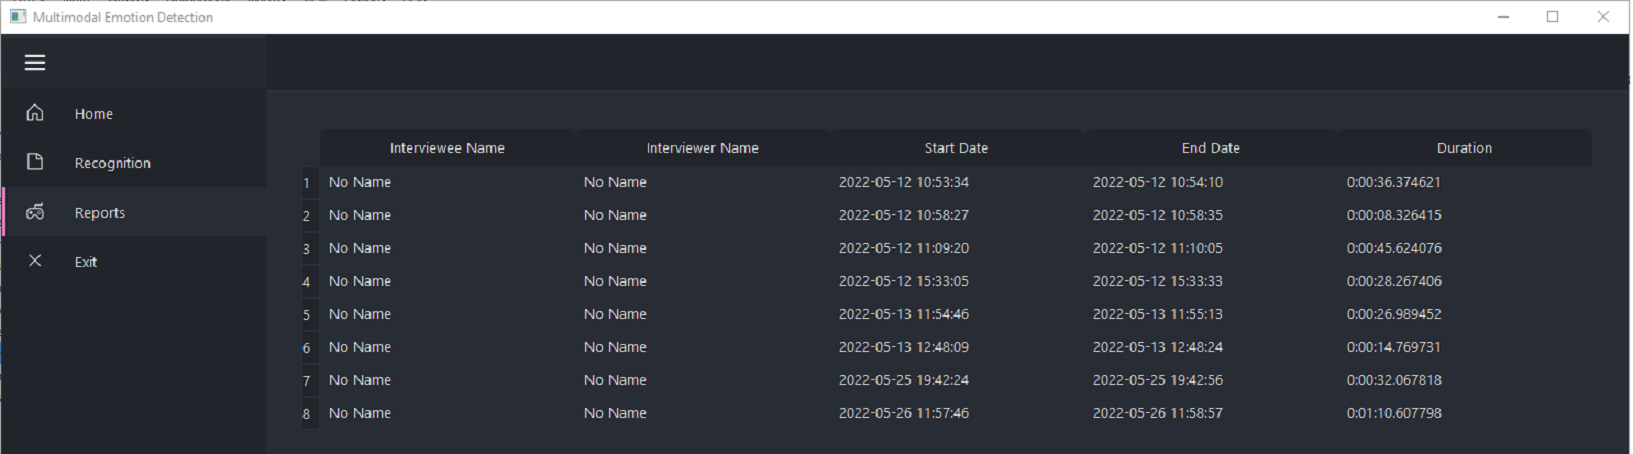
\includegraphics[scale=0.35]{images/reports.png}
		\end{center}
		\caption{Vizualizarea rapoartelor}
		\label{fig:emotion_reports}
	\end{figure}

	Din Figura \ref{fig:emotion_reports}, observăm denumirea coloanelor. Acestea sunt:
	
	\begin{itemize}
		\item Numele candidatului: pe baza acestui nume, rapoartele individului vor fi aduse din baza de date
		\item Numele persoanei care intervieveaza
		\item Data începerii interviului
		\item Data terminării interviului
		\item Durata interviului
	\end{itemize}
	
	De asemenea, se poate deschide un meniu contextual prin apăsarea click dreapta pe unul dintre rapoartele afișate. În cadrul acestei opțiuni, avem alegerea de a șterge raportul. În momentul în care se va dori ștergerea raportului, acesta va fi sters atât din baza de date, cât și din modul tabelar de vizualizare. Pentru vizualizarea într-o manieră amănunțită, putem face dublu click pe un raport, urmând ca fereastra să se comute pe una dedicată vizionării raportului.
	
	\clearpage
	\subsection{Vizualizare raport individual}
	În momentul schimbării în modul vizualizării de raport, vom fi întâmpinați de Figura \ref{fig:emotion_report}.
	
	\begin{figure}[H]
		\begin{center}
			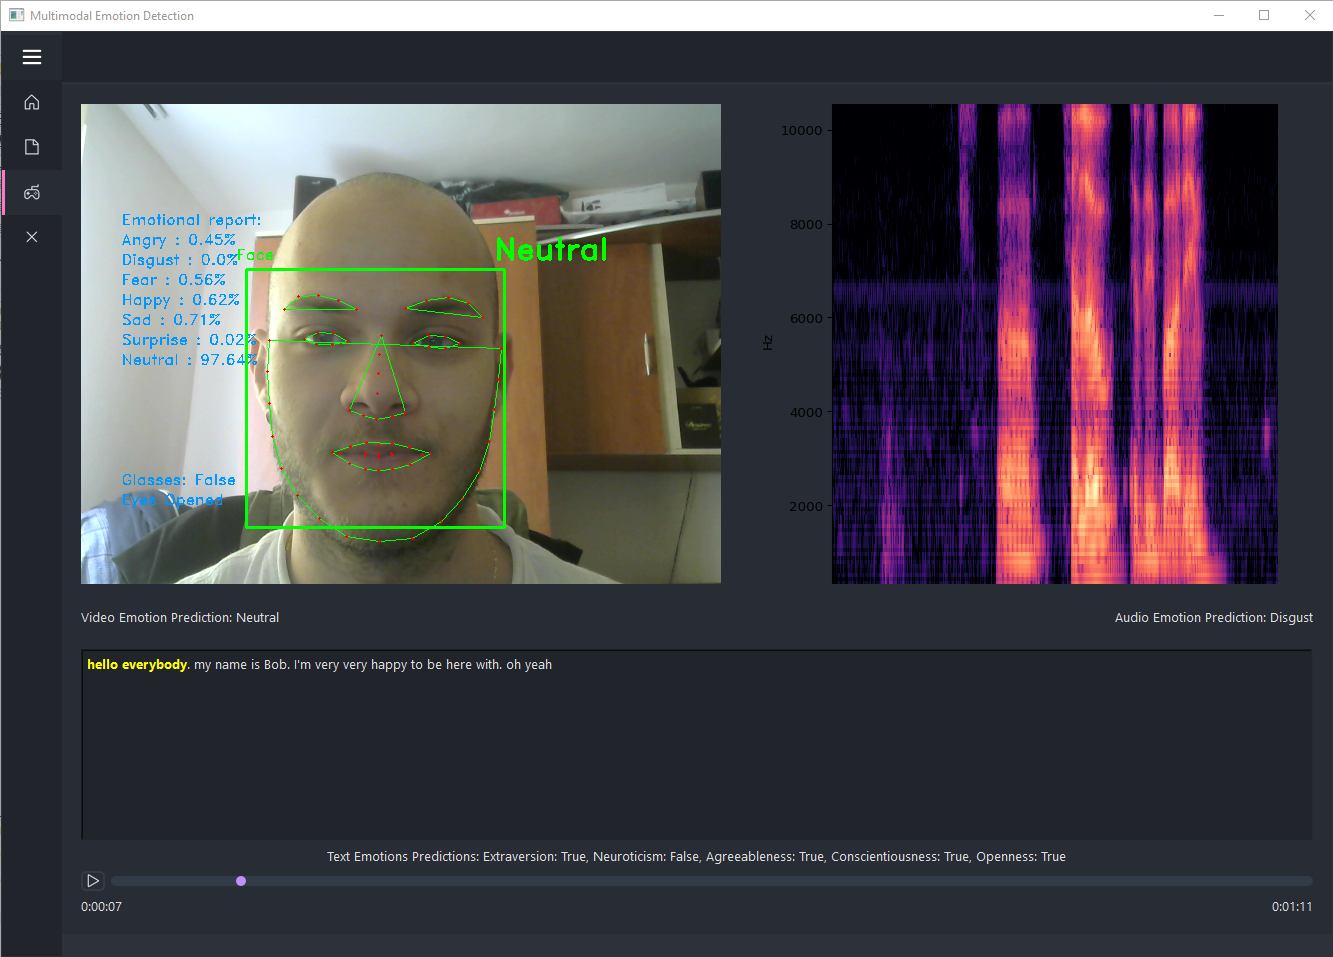
\includegraphics[scale=0.35]{images/emotion_report_visualize.png}
		\end{center}
		\caption{Vizualizarea raport}
		\label{fig:emotion_report}
	\end{figure}
	
	Elementele interactive din această fereastră sunt: glisorul, prin care se poate derula pe întreg interviul, precum și butonul pentru start/stop. În momentul interacționării cu raportul, se va crea un arbore, în care fiecare perspectivă de recunoașterea a emoțiilor vor fi stocate sub forma unor intervale. Având acces rapid datorită proprietăților oferite de arbori, ne vom putea folosi de glisor pentru a observa detalii din interviu.
	
	Pe lângă imaginea extrasă ca fiind cea mai sugestivă, este prezentată o etichetă, care să arate emoția prezisă de către modelul inteligent. În partea dreapta de fereastră video, putem observă o spectrogramă a intervalului audio. Este compusă din 4 secunde de date, având rolul de a evidenția anvelopa acustică, precum și degradarea sunetului. Asemănător etichetei pentru afișarea predicției video, putem observa o etichetă dedicată predicției audio.
	
	În funcție de mișcările glisorului, se va face evidențierea textului din intervalul dat (cu culoarea galbenă), identificat de către funcționalitate de speech-to-text. Deasupra glisorului se află cele 5 personalități precum și o valoare de adevăr, dacă valorile acestor indici trec de un anumit prag.
	
	\clearpage
	\subsection{Setări}
	Printre setările pe care le poate accesa utilizatorul (Fgura \ref{fig:settings}), enumerăm selectarea microfonului pe care dorim să îl utilizăm pentru detectarea emoțiilor precum și identificarea textului, numele candidatului și a persoanei care intervievează, precum și funcționalitățile de detectare a emoțiilor pe care dorim să le utilizăm.
	
	\begin{figure}[H]
		\begin{center}
			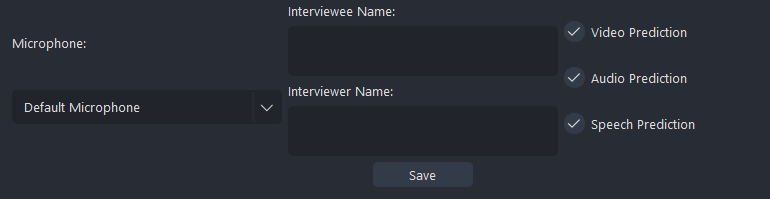
\includegraphics[scale=0.65]{images/settings.png}
		\end{center}
		\caption{Setările aplicației}
		\label{fig:settings}
	\end{figure}

	În funcție de modurile de identificare pe care dorim să le utilizăm, fereastra din Figura \ref{fig:emotion_recog} se va redimensiona astfel încât să se păstreze un aspect plăcut al interfeței grafice.
	
	\begin{figure}[H]
		\begin{center}
			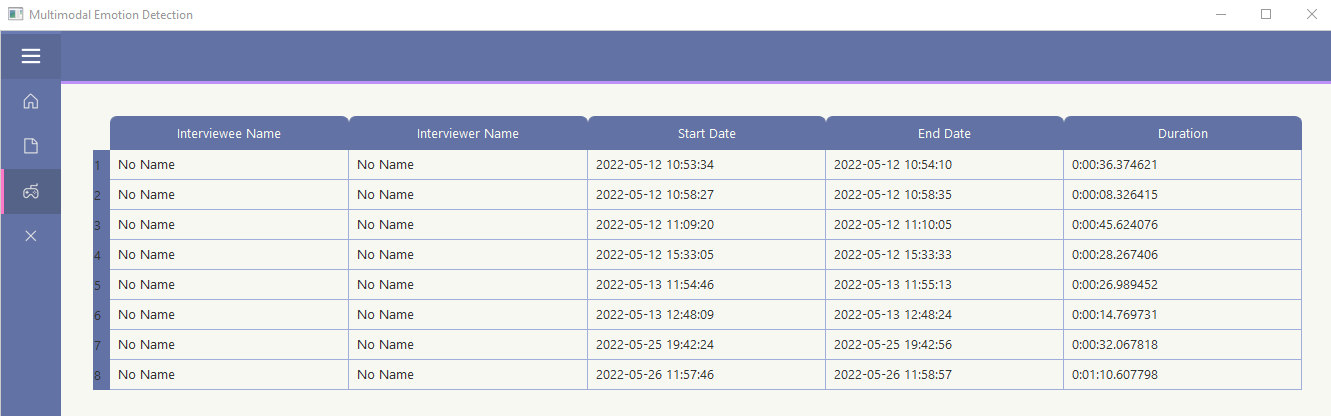
\includegraphics[scale=0.3]{images/light_theme.png}
		\end{center}
		\caption{Temă luminoasă}
		\label{fig:light_theme}
	\end{figure}
	
	Aplicația oferă disponibilitatea schimbărilor de aspect. Sunt oferite două teme: luminoasă și întunecată. În Figura \ref{fig:light_theme} se observă tema luminată, cu un aspect deschis la culoare care pune accent pe nuanța mov.

	Modul preferabil de utilizare al aplicației este acela de a lansa în execuție "Multimodal Emotion Detection" prin intermediul unui fișier bat. În timpul rulării fișierului, utilizatorul va fi interogat de tema pe care dorește să o folosească([d]ark/[l]ight). Este suficient de a introduce prima litera pentru a putea selecta tema dorită. În cazul în care utilizatorul introduce date invalide, va fi utilizată tema prestabilită, aceea fiind tema întunecată.

	\clearpage
	\section{Concluzii}
	Putem afirma faptul că utilizarea învățării automate în domeniul identificării emoțiilor în timp real este o abordare rar întâlnită și puțin explorată. Utilizând tehnici de procesare digitală de semnal (transformata Fourier pe termen scurt, spectrograme în scala Mel, fereastră Hamming), preprocesare de imagini și text, am fost capabili să putem antrena modele inteligente de învățare automată precum rețele neurale recurente sau convolutionale.

	Prin aplicația "Multimodal Emotion Detection" s-a realizat on interfață grafică în Qt, scrisă în limbajul de programare python, care vine în sprijinul identificării emoțiilor faciale, acustice și text în timpul realizării unui interviu. În cursul identificării emoțiilor, candidatul are feedback constant din partea aplicației, afișând prin intermediul interfeței grafice emoțiile identificate. 

	Automatul de stare adăugat în arhitectura aplicației are rolul de a restricționa accesul utilizatorului la anumite funcționalități, în concordanță cu starea care se află. Această limitare este impusă pentru a nu strica fluxul și modul de utilizare al aplicației. Cele trei butoane care fac posibilă comunicarea cu modurile de recunoaștere ale aplicației sunt administrate de către automatul de stare.

	Din punct de vedere personal, am realizat că învățarea automată aplicată identificării emoțiilor este o sarcină complexă, trecând peste așteptările pe care le-am setat. Primul obstacol pe care l-am întâmpinat a fost în înțelegerea modului în care o rețea ar putea identifica și recunoaște diferite șabloane în seturile de date. Emoțiile sunt mai complexe decât am putea să le înțeleagă un test pentru identificarea personalității sau o serie de actori care interpretează aceste emoții în mod artificial, fără vreun stimul extern. Al doilea obstacol întâlnit în procesul dezvoltării aplicației a fost cauzat de modul în care modelele ar putea executa recunoașterea în timp real, fără a se crea o decalare cu firul principal de execuție.

	Aceste obstacole au fost depășite cu succes, și mai mult decât atât, s-a oferit prilejul de a dezvolta un mod de vizualizare a 	rapoartelor generate în urma terminării interviurilor. Fiind un mod interactiv de vizualizare, se poate analiza fiecare segment creat, datorită proprietăților oferite de intervale, modul de stocare al datelor la acest nivel. Într-un nivel mai superior, datele fiind stocate în MongoDb, ne oferă un suport nativ pentru interogarea lor.

	Însă întotdeauna este loc îmbunătățire. Printre direcțiile care se doresc a fi implementate, se vizează:
	
	\begin{itemize}
		\item consolidarea performanței și a acurateței oferite de către modelele de identificare a emoțiilor;
		\item migrarea aplicației într-o interfață web, pentru a nu solicita calculatorul utilizatorului;
		\item adăugarea unui modul de înregistrare și autentificare a utilizatorilor.
	\end{itemize}
	
	\clearpage
    \printbibliography
    \clearpage
	\begin{figure}[H]
		\begin{center}
			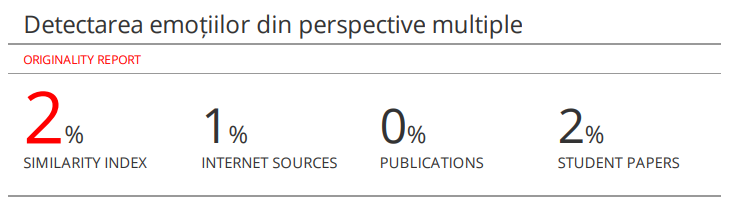
\includegraphics[scale=0.8]{images/plagiat.PNG}
		\end{center}
		\caption{Disertație similaritate}
		\label{fig:sim}
	\end{figure} 	
\end{document}